% ============================================== %
% Author: Andrea Spinelli
%
% Thesis Title: Allineamento, Denoising e Stacking di Immagini lunari mediante tecniche tradizionali e Unsharp Masking basato su Deep Learning
% 
% Laurea in Ingegneria Informatica e Automatica, Università di Roma La Sapienza.
%
% https://github.com/Spina02/Thesis
%
% ============================================== %

% Document Class
\documentclass[noexaminfo, oneside]{sapthesis} % binding=0.6cm, 

% Packages
\usepackage{microtype}
\usepackage[italian, provide=*]{babel}
\usepackage[T1]{fontenc}
\usepackage[utf8]{inputenc}
\usepackage{hyperref}
\usepackage{listings}
\usepackage[dvipsnames]{xcolor}
\usepackage{xspace}
\usepackage{geometry} 
\usepackage{caption}  
\usepackage[edges]{forest}
\usepackage{subcaption}
\usepackage{float}    
\usepackage{lipsum}  
\usepackage{xargs}              
\usepackage{booktabs}
\usepackage{graphicx}
\usepackage{makecell}
\usepackage{booktabs}
\usepackage{tabularx}
\usepackage{longtable}
\usepackage{threeparttable}
\usepackage{amsthm}
\usepackage{amssymb}
\usepackage{amsmath}
\usepackage[Algoritmo]{algorithm}      
\usepackage{algpseudocode}
\counterwithin{algorithm}{chapter}
\usepackage[colorinlistoftodos,prependcaption,textsize=tiny]{todonotes}
\usepackage{csquotes}
\usepackage{enumitem}
\usepackage[noabbrev,capitalize,nameinlink,italian]{cleveref}
\creflabelformat{equation}{#2\textup{#1}#3}
\usepackage{mathrsfs}
\newcommand\sbullet[1][.75]{\mathbin{\vcenter{\hbox{\scalebox{#1}{$\bullet$}}}}}
\usepackage{leftindex}

\usepackage[
  backend=bibtex,
  style=numeric,
  sorting=anyt,
  minnames=1,
  maxnames=1,
  minalphanames=3,
]{biblatex}

\usepackage{listings}
\usepackage{xcolor}

% Commands and Settings
\newcommandx{\unsure}[2][1=]{\todo[linecolor=red,backgroundcolor=red!25,bordercolor=red,#1]{#2}}
\newcommandx{\change}[2][1=]{\todo[linecolor=blue,backgroundcolor=blue!25,bordercolor=blue,#1]{#2}}
\newcommandx{\info}[2][1=]{\todo[linecolor=OliveGreen,backgroundcolor=OliveGreen!25,bordercolor=OliveGreen,#1]{#2}}
\newcommandx{\improvement}[2][1=]{\todo[linecolor=Plum,backgroundcolor=Plum!25,bordercolor=Plum,#1]{#2}}
\newcommandx{\thiswillnotshow}[2][1=]{\todo[disable,#1]{#2}}
\newcolumntype{L}[1]{>{\raggedright\arraybackslash}p{#1}}
\newcounter{boxlblcounter}  
\newcommand{\makeboxlabel}[1]{\fbox{#1.}\hfill}
\newenvironment{boxlabel}
  {\begin{list}
    {\arabic{boxlblcounter}}
    {\usecounter{boxlblcounter}
     \setlength{\labelwidth}{3em}
     \setlength{\labelsep}{0em}
     \setlength{\itemsep}{2pt}
     \setlength{\leftmargin}{1.5cm}
     \setlength{\rightmargin}{2cm}
     \setlength{\itemindent}{0em} 
     \let\makelabel=\makeboxlabel
    }
  }
{\end{list}}
\lstdefinestyle{myStyle}{
  language=Python,
  basicstyle=\ttfamily\footnotesize,
  keywordstyle=\color{blue!40!black}\bfseries,
  commentstyle=\itshape\color{green!40!black},
  stringstyle=\color{red!40!black},
  showstringspaces=false,
  numbers=left,
  numberstyle=\tiny\color{gray},
  stepnumber=1,
  frame=single,
  breaklines=true,
  tabsize=2,
  numbersep=-10pt,
  captionpos=b,
  belowcaptionskip=1\baselineskip,
  frame = tb,
  identifierstyle=\color{black},
  backgroundcolor=\color{white},
}
\lstset{style=mystyle}

\setlength{\parindent}{0pt}
\setlength{\parskip}{5pt}

% Metadata
\definecolor{sapienzared}{HTML}{000000}
\hypersetup{pdftitle={Thesis},pdfauthor={Andrea Spinelli}, urlcolor=sapienzared, linkcolor=sapienzared, colorlinks=true, citecolor=sapienzared}
\title{Allineamento, Denoising e Stacking di immagini $\\$lunari mediante tecniche tradizionali e Unsharp $\\$Masking basato su Deep Learning}
\author{Andrea Spinelli}
\IDnumber{1985877}
\course{Laurea Triennale in Ingegneria Informatica}
\courseorganizer{Facoltà di Ingegneria dell'Informazione, Informatica e Statistica}
\AcademicYear{2023/2024}
\advisor{Prof. Thomas Alessandro Ciarfuglia}
\authoremail{andreaspinelli2002@gmail.com}
\copyyear{2024}
\thesistype{Laurea Triennale}

% ================== CUSTOM ENVIRONMENTS ==================

\newtheorem{lemma}{Lemma}[chapter]

\theoremstyle{definition}
\newtheorem{definition}{Definition}[chapter]

\theoremstyle{definition}
\newtheorem{example}{Example}[chapter]

\newtheorem{theorem}{Theorem}[chapter]

% ================== CUSTOM MACROS ==================

\newcommand{\curlyquotes}[1]{\textquotedblleft #1\textquotedblright}
\newcommand{\abs}[1]{\left|#1\right|}
\newcommand{\rbk}[1]{\left(#1\right)}
\newcommand{\abk}[1]{\left\langle#1\right\rangle}
\newcommand{\soe}[2]{\left\{\begin{array}{#1} #2 \end{array}\right.}
\DeclareMathOperator*{\argmax}{arg\,max}
\newcommand{\sbk}[1]{\left[#1\right]}
\newcommand{\resizable}[2]{\resizebox{#1\hsize}{!}{#2}}
\newcommand{\centeredeq}[2]{\begin{equation*}\resizable{#1}{#2}\end{equation*}}
\newcommand{\centeredsoe}[1]{\left . \begin{array}{c} #1 \end{array} \right .}
\algdef{SE}[DOWHILE]{Do}{doWhile}{\algorithmicdo}[1]{\algorithmicwhile\ #1}%
\newcommand{\say}[1]{\flqq\textit{#1}\frqq}
\newcommand{\NPclass}{\textsf{NP}\xspace}
\newcommand{\NPHard}{\textsf{NP-Hard}\xspace}
\newcommand{\NPComplete}{\textsf{NP-Complete}\xspace}
\newenvironment{nocaptionalg} % environment for algorithms without caption
{
    \par\addvspace{\topsep}
    \centering
    \begin{minipage}{\linewidth}
    \hrule\kern2pt
}
{
    \par\kern2pt\hrule
    \end{minipage}
    \par\addvspace{\topsep}
}

% ================== DOCUMENT ==================

\addbibresource{./references.bib}

\begin{document}

\lstset{language=Python}

\frontmatter

\maketitle

% ================== DEDICATION ==================

\dedication{
  \say{Tutta colpa della Luna, quando si avvicina troppo alla Terra fa impazzire tutti}\\― William Shakespeare
}

% ================== ABSTRACT ==================

\begin{abstract}
    In questa relazione viene presentato lo sviluppo di un software per l'elaborazione di immagini lunari, combinando tecniche tradizionali di image processing con approcci all'avanguardia basati su deep learning. Il progetto implementa un workflow completo e automatizzato che include calibrazione delle immagini raw, allineamento automatico tramite feature detection e matching, riduzione del rumore mediante DnCNN (Denoising Convolutional Neural Network), aumento della nitidezza tramite Unsharp Masking e diversi metodi di stacking per la creazione di immagini finali ad alta qualità.
    
    Particolare attenzione è stata dedicata allo sviluppo di un algoritmo di Unsharp Masking personalizzato che integra DnCNN con maschere basate sul gradiente dell'immagine. Questo approccio innovativo permette di preservare i dettagli significativi durante la riduzione del rumore, evitando la tipica perdita di informazioni che caratterizza i metodi tradizionali. Il sistema è stato testato su un dataset di immagini lunari acquisite con una fotocamera bridge Fujifilm FinePix S1, dimostrando come sia possibile ottenere risultati di qualità professionale anche con attrezzatura amatoriale, rendendo l'astrofotografia più accessibile.
    
    La valutazione quantitativa dei risultati è stata effettuata utilizzando multiple metriche di qualità dell'immagine senza riferimento, tra cui BRISQUE (Blind/Referenceless Image Spatial Quality Evaluator), NIQE (Natural Image Quality Evaluator) e LIQE (Learning-based Image Quality Evaluator). I risultati sperimentali hanno evidenziato miglioramenti significativi nelle diverse fasi di elaborazione, con particolare efficacia nella riduzione del rumore e nel recupero dei dettagli superficiali lunari. Il progetto fornisce una solida base per futuri sviluppi nell'ambito dell'elaborazione automatica di immagini astronomiche, con possibili applicazioni in altri contesti di imaging scientifico.
\end{abstract}

\let\cleardoublepage\clearpage


\cleardoublepage

\tableofcontents
\let\cleardoublepage\clearpage

\mainmatter

% ================== CHAPTERS ==================

\definecolor{sapienzared}{HTML}{812333}

\chapter{Introduzione} \label{chap:introduction}

\section{Evoluzione dell'astrofotografia} \label{sec:evolution}

L'\textbf{\href{https://it.wikipedia.org/wiki/Astrofotografia}{astrofotografia}} si occupa di fotografare oggetti celesti come stelle, pianeti, galassie e nebulose. Questa pratica ha radici risalenti al XIX secolo: nel 1822 fu scattata la prima foto nella storia da Nicéphore Niépce, e già nel 1840 John William Draper catturò la prima immagine della Luna, segnando l'inizio di una nuova era nell'osservazione astronomica. Nel 1850, William Cranch Bond e John Adams Whipple scattarono la prima fotografia di una stella, \textit{Vega}, con un'esposizione di 1000 secondi.

\subsection{Breve storia e sviluppo tecnologico} \label{subsec:history}

Nei primi anni le immagini erano ottenute con \textit{lastre fotografiche di vetro}, che richiedevano tempi di esposizione estremamente lunghi. Catturare immagini di oggetti deboli come nebulose e galassie era un'impresa ardua e poteva richiedere ore o notti intere di esposizione, rendendo il processo molto laborioso. Le prime immagini si concentravano infatti su oggetti luminosi, come la Luna e i pianeti, mentre stelle più deboli e galassie rimanevano al di là delle capacità tecnologiche dell'epoca \cite{astroph_hist}. 
Con la nascita della \textit{fotografia a colori} gli astronomi potettero registrare le diverse tonalità di colore degli oggetti celesti, rendendo possibile ottenere informazioni circa la composizione chimica e la temperatura di stelle e nebulose. La vera rivoluzione arrivò con l'avvento della \textbf{\href{https://it.wikipedia.org/wiki/Fotografia_digitale}{fotografia digitale}} e l'introduzione di \textit{dispositivi a carica accoppiata} (\textit{CCD}) alla fine degli anni '60. I \textit{CCD} avevano sensibilità alla luce notevolmente superiore rispetto alle lastre fotografiche, permettendo tempi di esposizione più brevi e maggiore qualità dell'immagine. Ciò consentì di rilevare oggetti celesti più deboli e ridurre significativamente il rumore nelle immagini \cite{multiwavelength_image_proc}.

Con la diffusione dei computer, l'elaborazione delle immagini digitali divenne parte integrante dell'astrofotografia. Tecniche come la \textit{calibrazione}, l'\textit{allineamento}, la \textit{riduzione del rumore} e lo \textit{stacking} delle immagini hanno permesso di ottenere risultati di qualità superiore rispetto alle immagini singole. L'utilizzo di algoritmi avanzati consentì di rivelare dettagli nascosti, migliorare il  contrasto e ridurre al minimo il rumore aumentando l'accuratezza delle osservazioni astronomiche \cite{calibration}.

Oggi l'astrofotografia è accessibile non solo ad astronomi professionisti, ma anche ad appassionati dilettanti. L'ampia disponibilità di telescopi, fotocamere e software avanzati ha reso possibile catturare immagini di alta qualità anche con strumenti di costo contenuto. L'astrofotografia è diventata un hobby popolare tra appassionati di astronomia e fotografia, che condividono le proprie immagini e scoperte sui social e forum online come \textit{\href{https://www.cloudynights.com/index}{Cloudy Nights}} o \textit{\href{https://www.astrobin.com}{AstroBin}}.

\section{Stato dell'arte: strumentazione e tecniche moderne} \label{sec:state_of_the_art}

L'astrofotografia moderna si avvale di strumenti sofisticati e tecniche avanzate per catturare immagini di alta qualità. I telescopi sono dotati di montature motorizzate che compensano il movimento apparente del cielo, consentendo esposizioni più lunghe senza sfocature. Le fotocamere digitali, spesso equipaggiate con sensori \textit{CCD} o \textit{CMOS}, sono in grado di catturare immagini ad alta risoluzione anche di oggetti celesti deboli quali galassie o nebulose, preservandone i dettagli. I software di elaborazione delle immagini offrono strumenti avanzati per la calibrazione, l'allineamento e la post-produzione delle immagini, consentendo di ottenere risultati di qualità professionale.

\begin{figure}[H]
    \centering
    \includegraphics[scale = 0.6]{../assets/Webb_POC.jpg}
    \captionsetup{justification=centering}
    \caption{\textit{Pillars of Creation}, \textit{Nebulosa dell'Aquila}, ripresi dal \textit{James Webb} combinando dati acquisiti da \textit{NIRCam} e \textit{MIRI}. Immagine originale disponibile su \cite{webb_telescope}} \label{fig:webb_poc}
\end{figure}

Esistono diversi telescopi spaziali, come l'\textit{\href{https://hubblesite.org/home}{Hubble Space Telescope}} \cite{hubble} della \textit{NASA} e il \textit{\href{https://webbtelescope.org/home}{James Webb Space Telescope}} \cite{jwst}, gestito congiuntamente da \textit{ESA}, \textit{NASA} e \textit{CSA}. Questi strumenti, orbitando al di fuori dell'atmosfera terrestre, sono in grado di catturare immagini ad altissima risoluzione e sensibilità, libere dalle distorsioni e dall'inquinamento luminoso terrestre. Sfruttano a proprio vantaggio fenomeni fisici come le \textit{lenti gravitazionali} e la \textit{diffrazione} per osservare oggetti nello spazio profondo, ben oltre le capacità degli strumenti terrestri. Questi telescopi, inoltre, sono dotati di telecamere come la \textit{NIRCam} (Near Infrared Camera) e la \textit{MIRI} (Mid Infrared Instrument), che permettono di osservare l'universo in bande di luce altrimenti invisibili, rivelando dettagli nascosti e processi fisici altrimenti inaccessibili (\cref{fig:webb_poc}), e si dimostrano fondamentali per la ricerca astronomica.

\subsection{Hardware} \label{subsec:hardware}

Nell'astrofotografia tradizionale si utilizzano principalmente tre tipi di strumenti:

\begin{itemize}
    \item \textbf{Telescopi}: I telescopi sono fondamentali nell'astrofotografia; ne esistono di diversi tipi, tra cui rifrattori, riflettori e catadiottrici, ciascuno con caratteristiche specifiche. I telescopi moderni variano da piccoli modelli portatili a grandi strutture professionali, come l'\textit{\href{https://elt.eso.org/}{ELT}} (Extremely Large Telescope), con uno specchio principale di ben $ 39 \text{m} $ di diametro, che è ancora in costruzione ma si prevede diventerà operativo entro il 2027 \cite{elt}. La scelta del telescopio dipende dall'oggetto celeste da osservare e dal livello di dettaglio desiderato, oltre che dal budget disponibile.

    \item \textbf{Fotocamere}: Le fotocamere \textit{\textbf{CCD}} (Charge-Coupled Device) sono ampiamente utilizzate in ambito astronomico per la loro alta sensibilità e basso \hyperref[sec:noise]{rumore elettronico}. Negli ultimi anni, le fotocamere \textit{\textbf{CMOS}} (Complementary Metal-Oxide-Semiconductor) hanno guadagnato popolarità in quanto più performanti e più accessibili economicamente. Tali fotocamere offrono elevate risoluzioni, velocità di lettura più rapide e buona \href{https://it.wikipedia.org/wiki/Efficienza_quantica}{\textit{efficienza quantica}}, rendendole adatte sia per l'uso professionale che amatoriale \cite{image_processing}.
    
    \item \textbf{Montature}: Una montatura stabile e precisa è essenziale per compensare la rotazione terrestre durante le lunghe esposizioni.

    \begin{itemize}
        \item Le \textit{montature equatoriali} sono progettate per seguire il movimento apparente delle stelle nel cielo, consentendo di mantenere gli oggetti celesti centrati nell'inquadratura.
        \item Le \textit{montature altazimutali}, più semplici da utilizzare, richiedono sistemi di derotazione o software di correzione più sofisticati per lunghe esposizioni, a causa della rotazione di campo.
        \item Le \textit{montature computerizzate}, dotate di sistemi \textit{GoTo}, permettono di puntare automaticamente verso specifici oggetti celesti e di tracciarli con precisione.
    \end{itemize}

\end{itemize}

\subsection{Software e algoritmi nell'astrofotografia} \label{subsec:software}

Con il tempo i software utilizzati in ambito astrofotografico sono arrivati al punto tale per cui non è necessario essere dotati di un \hyperref[subsec:hardware]{hardware} professionale per catturare immagini di corpi celesti anche dal proprio cortile (o \textit{"from my backyard"}).

I software principalmente utilizzati, quali \href{https://pixinsight.com/}{\textit{PixInsight}} o \href{https://www.autostakkert.com/}{\textit{AutoStakkert}} implementano diversi algoritmi in grado di migliorare sensibilmente i risultati finali:

\begin{itemize}
\item \textbf{Calibrazione delle immagini}: La calibrazione è un passaggio cruciale per rimuovere artefatti e rumori dovuti alla strumentazione dalle immagini astronomiche. Questo processo utilizza diversi insiemi di frame di calibrazione: \textit{bias frames, dark frames} e \textit{flat frames} (più nel dettaglio nella \cref{sec:calibration}) dai quali è possibile estrarre informazioni sul rumore dell'immagine, così da poterlo sottrarre alla stessa \cite{calibration}.

\item \textbf{Allineamento delle immagini}: L'allineamento è necessario per combinare correttamente più immagini dello stesso oggetto. Algoritmi di feature detection come \textit{\textbf{ORB}} (Oriented FAST and Rotated BRIEF) \cite{orb}, \textit{\textbf{SIFT}} (Scale-Invariant Feature Transform) e \textit{\textbf{SURF}} (Speeded Up Robust Features) identificano punti caratteristici nelle immagini per calcolare \hyperref[subsec:homography]{\textit{trasformazioni omografiche}}, utilizzate per correggere differenze di scala, rotazione e prospettiva tra le immagini (più nel dettaglio nella \cref{sec:alignment}) \cite{multiwavelength_image_proc} \cite{improved_solan}.

\item \textbf{Riduzione del rumore}: La riduzione del rumore migliora la qualità finale delle immagini. Tecniche tradizionali come l'unsharp masking \cite{multiwavelength_image_proc} accentuano i dettagli sottraendo una versione sfocata dell'immagine originale. Approcci più avanzati utilizzano reti neurali convoluzionali profonde, come \textit{\textbf{DnCNN}} (Denoising Convolutional Neural Network) \cite{DnCnn}, che apprendono a rimuovere il rumore preservando i dettagli attraverso l'addestramento su grandi dataset (più nel dettaglio nelle sezioni \ref{sec:preprocessing} e \ref{sec:postprocess}).

\item \textbf{Stacking delle immagini}: Lo \textit{stacking} (\textit{"impilamento"}) combina multiple esposizioni per ottenere un'unica immagine finale ottimizzandone il rapporto segnale-rumore. Questa tecnica riduce il rumore casuale e mette in evidenza dettagli deboli non visibili in singole esposizioni. Metodi come il \textbf{\textit{Weighted Average Stacking}} assegnano un peso a ciascuna immagine in base ad un criterio prefissato, per ottenere in seguito un'immagine data dalla media ponderata dei valori dei singoli frames in input (più nel dettaglio nella \cref{sec:stacking}).
\end{itemize}

\section{Rumore e artefatti nelle immagini astronomiche} \label{sec:noise}

La qualità delle immagini astronomiche è influenzata da diversi tipi di rumore e artefatti, che devono essere mitigati per ottenere risultati ottimali (vedremo nella \cref{subsec:denoising} come ridurli). I principali tipi di rumore e artefatti includono:

\begin{itemize}
    \item \textbf{Rumore termico}: Il rumore termico (\textit{Dark Current}) è generato dall'agitazione termica degli elettroni all'interno del sensore della fotocamera, producendo un segnale anche in assenza di luce. Questo tipo di rumore aumenta con la temperatura del sensore ed è particolarmente significativo nelle lunghe esposizioni. Per ridurlo, molti sensori astronomici sono raffreddati tramite \textit{sistemi termoelettrici} o \textit{criogenici}. La sottrazione dei \hyperref[subsec:dark]{\textit{dark frames}} durante la calibrazione permette di correggere questo rumore.
    
    \item \textbf{Rumore del sensore}: Include diversi tipi di rumore intrinseco al sensore della fotocamra:
    
    \begin{itemize}
        \item \textbf{Rumore di lettura}: deriva dall'elettronica durante il processo di lettura e digitalizzazione del segnale dal sensore. È generalmente costante e può essere minimizzato utilizzando componenti elettronici di alta qualità. Sebbene il rumore di lettura non possa essere eliminato, l'uso di \hyperref[subsec:bias]{\textit{bias frames}} nella calibrazione aiuta a compensare l'offset introdotto dall'elettronica.
        
        \item \textbf{Rumore di schema fisso}: Il rumore di schema fisso (\textit{Fixed Pattern Noise}) è causato dalle variazioni di sensibilità tra i pixel, si manifesta come pattern ripetuti nell'immagine. L'utilizzo dei \hyperref[subsec:flat]{\textit{flat frames}} nella calibrazione aiuta a correggere queste imperfezioni.
        
        \item \textbf{Amp glow}: È una luminescenza causata dal calore generato dai circuiti di amplificazione del sensore, visibile come un bagliore ai bordi dell'immagine. La sottrazione dei \hyperref[subsec:dark]{\textit{dark frames}} e il raffreddamento del sensore contribuiscono a ridurre questo fenomeno.
    \end{itemize}
    
    \item \textbf{Altri artefatti}: altri artefatti includono la vignettatura, un oscuramento ai bordi dell'immagine dovuto alle caratteristiche ottiche del sistema e mitigabile con i \hyperref[subsec:flat]{\textit{flat frames}}, e i \textit{pixel caldi e morti},  ossia pixel che rimangono sempre accesi o spenti, che possono essere mappati e corretti durante l'elaborazione.

\end{itemize}

\section{La Luna} \label{sec:moon}

\begin{figure}[H]
    \centering
    \includegraphics[scale = 0.35]{../assets/moonrota.png}
    \captionsetup{justification=centering}
    \caption{Dimostrazione grafica del moto di rotazione e rivoluzione della Luna \cite{moon_rota}} \label{fig:moonrota}
\end{figure}

Tra i corpi celesti più affascinanti e accessibili nell'astrofotografia spicca sicuramente la \textbf{Luna}. Grazie alla sua vicinanza alla Terra, alla sua luminosità e alle sue dimensioni apparenti relativamente grandi, è possibile catturare immagini lunari di alta qualità anche in assenza di strumentazione professionale. Fotografare la Luna rispetto ad altri corpi celesti presenta diversi vantaggi:

\begin{itemize}
    \item \textbf{Rotazione sincrona}: La Luna mostra sempre la stessa faccia verso la Terra a causa della sua \textit{rotazione sincrona}, ovvero il suo periodo di rotazione attorno al proprio asse è uguale al periodo di rivoluzione attorno alla Terra (circa 27,3 giorni) [\cref{fig:moonrota}]. Questo fenomeno, dovuto alla \textit{risonanza mareale}, comporta diverse semplificazioni nell'elaborazione delle immagini, eliminando la necessità di processi di derotazione \cite{nasa_moon_orbit}.
    
    \item \textbf{Luminosità elevata}: La Luna è l'oggetto celeste più luminoso nel cielo notturno. Questa luminosità consente di utilizzare tempi di esposizione più brevi rispetto ad altri oggetti astronomici (da $1/250$ a $1/100$ di secondo, a seconda della percentuale di illuminazione, contro tempi fino a $20$-$30$ secondi per oggetti dello spazio profondo), riducendo gli effetti del \hyperref[sec:noise]{rumore elettronico} e del movimento apparente.
    
    \item \textbf{Facilità di localizzazione}: Essendo facilmente visibile ad occhio nudo, la Luna non richiede sistemi di puntamento sofisticati o montature equatoriali per essere fotografata. Un semplice treppiede è sufficiente per stabilizzare la fotocamera durante la cattura delle immagini.
\end{itemize}

Nell'astrofotografia planetaria in generale, quando il soggetto non è la Luna, i pianeti sono notevolmente distanti dalla Terra, e piccole perturbazioni dell'atmosfera possono causare rumore e artefatti fastidiosi. È possibile ovviare a questo problema registrando dei video (piuttosto che singole immagini) e rimuovere tali artefatti tramite una tecnica chiamata \textit{Lucky Imaging}, combinata con tecniche di \textit{derotazione} per mitigare l'effetto della rotazione del pianeta attorno al proprio asse.

L'astrofotografia lunare professionale consiste spesso nello scattare immagini che catturano sezioni diverse della Luna; queste vengono prima processate singolarmente e poi unite mediante tecniche di \textit{stitching}. Un'altra tecnica molto diffusa è quella utilizzata per ottenere le cosiddette \textit{Mineral Moon}: si eseguono diversi scatti applicando filtri a banda stretta sui telescopi, per poi elaborare i canali RGB singolarmente, facendo risaltare la presenza di minerali diversi sulla superficie lunare \cite{legault_astrophoto}.

Fotografare la Luna presenta anche diverse sfide. Essa è caratterizzata da un elevato contrasto tra le aree illuminate e quelle in ombra, specialmente durante le fasi parziali, rendendo difficile ottenere un'esposizione bilanciata che catturi dettagli in entrambe le zone \cite{sheehan_epic_moon}. Nonostante la sua vicinanza, l'atmosfera terrestre influenza la qualità delle immagini lunari, introducendo turbolenze (\textit{seeing}), dispersione e attenuazione della luce, portando ad una riduzione di nitidezza e contrasto nei risultati \cite{sheehan_epic_moon}. Infine, sebbene la luminosità della Luna consenta di fotografarla anche da aree urbane, l'inquinamento luminoso può ancora influenzare la qualità, specialmente quando si vuole catturare dettagli più fini o nelle le fasi meno illuminate.

Nel contesto di questo progetto, sono state scattate personalmente immagini della Luna utilizzando una \textbf{Fujifilm FinePix S1}, una fotocamera bridge dotata di uno zoom ottico fino a $50 \times$. Senza l'ausilio di telescopi o montature specializzate, ma semplicemente con l'utilizzo di un treppiede standard, è stato possibile catturare immagini dettagliate della superficie lunare.

Questa scelta evidenzia come, grazie alle moderne tecnologie e alle tecniche di elaborazione delle immagini, sia possibile ottenere risultati di qualità anche con attrezzature relativamente modeste. Le immagini acquisite sono state utilizzate per testare e validare gli algoritmi sviluppati nel corso del progetto, dimostrando l'efficacia delle metodologie proposte nell'ottimizzazione di fotografie lunari.
\cleardoublepage
\chapter{Elaborazione di immagini lunari} \label{chap:techniques}

Questo capitolo si propone di approfondire le tecniche di elaborazione delle immagini lunari, illustrando le nozioni teoriche alla base degli algoritmi implementati nel progetto. Ogni tecnica verrà descritta in dettaglio, partendo da calibrazione e allineamento, passando per pre-processing e stacking, per concludere con il post-processing. Quando necessario, verranno forniti pseudocodice e descrizioni dei processi matematici applicati alle immagini; l'implementazione sarà invece discussa nel capitolo \ref{chap:implementation}.

\section{Calibrazione di immagini} \label{sec:calibration}

La \textbf{calibrazione} delle immagini è un passaggio fondamentale nell'astrofotografia, necessario per rimuovere rumore e artefatti introdotti dalla strumentazione. In particolare, nel contesto delle immagini lunari, la calibrazione è utile per rimuovere il rumore termico e i difetti del sensore, oltre a uniformare l'illuminazione dell'immagine. Questo processo è composto da tre fasi principali: la cattura di \textit{bias frames}, \textit{dark frames} e \textit{flat frames}. Tali scatti devono essere acquisiti con la fotocamera nello stesso stato in cui sono state scattate le immagini lunari, in particolare nelle stesse condizioni termiche. Infatti, quando viene eseguita una sessione di molti scatti, o con lunghe esposizioni, la macchinetta tende a scaldarsi causando effetti non sempre trascurabili, e sono proprio quelli che vogliamo mitigare mediante la fase di calibrazione. In questa fase gli scatti della luna vengono denominati \textit{light frames}  \cite{calibration}.

\subsection{Bias Frames} \label{subsec:bias}

I \textbf{bias frames} son scatti acquisiti con il tempo di esposizione più breve possibile (il minimo supportato dalla macchina fotografica, idealmente zero), ISO uguale a quello dei light frames e con l'otturatore della fotocamera chiuso. Questi frame catturano il \textbf{rumore di bias}, un segnale di offset introdotto dall'elettronica del sensore in assenza di luce. Il rumore di bias è presente in tutte le immagini acquisite con una macchina fotografica, e varia leggermente da pixel a pixel.

Per correggere questo rumore si calcola il cosiddetto \textbf{master bias} combinando i diversi bias frames, generalmente calcolandone la media. Il master bias viene poi sottratto da tutte le immagini acquisite, inclusi gli altri frame di calibrazione.

\begin{algorithm}[H]
    \caption{\texttt{- Calcolo del master bias}:\\ Data la lista di bias frames $B_f$, l'algoritmo calcola il master bias $M_b$} \label{alg:bias}
    \begin{algorithmic}[1]
        \Function{calculate\_master\_bias}{$B_f$}
            \State $N \gets$ \text{numero di bias frames}
            \State $M_b \gets 0$
            \For{$i \gets 1$ to $N$}
                \State $M_b \gets M_b + \dfrac{B_f[i]}N$ \Comment{Media dei bias frames}
            \EndFor
            \State \textbf{return} $M_b$
        \EndFunction
    \end{algorithmic}
\end{algorithm}

\textbf{Applicazione:} Per applicare il master bias a un'immagine, si sottrae semplicemente il master bias dall'immagine originale. In formula, data un'immagine \textit{original} e il master bias \textit{master\_bias}, l'immagine calibrata \textit{final\_image} sarà data da:

$$
    final\_image = original - master\_bias
$$

\subsection{Dark Frames} \label{subsec:dark}

I \textbf{dark frames}, acquisiti con stessi ISO e tempi di cattura dei light frames, ma con l'otturatore chiuso, catturano il \textbf{rumore termico} causato dall'agitazione termica degli elettroni nel sensore. Questo rumore aumenta con il tempo di esposizione e con la temperatura del sensore e può variare significativamente tra scatti differenti.

Per correggere il rumore termico, si calcola il \textbf{master dark} combinando i diversi dark frames, generalmente calcolandone la media. Il master dark viene poi sottratto ai light frames e ai flat fames. È importante sottrarre il master bias dai dark frames prima di calcolare il master dark, per evitare di sommare due volte il rumore di bias.

\begin{algorithm}[H]
    \caption{\texttt{- Calcolo del Master Dark}:\\ Data la lista di dark frames $D_f$ e il master bias $M_b$, l'algoritmo calcola il master dark $M_d$.} \label{alg:dark}
    \begin{algorithmic}[1]
        \Function{calculate\_master\_dark}{$D_f$, $M_b$}
            \State $N \gets$ \text{numero di dark frames}
            \State $M_d \gets 0$
            \For{$i \gets 1$ to $N$}     
                \State $ D_c \gets D_f[i] - M_b$ \Comment rimozione del bias
                \State $M_d \gets M_d + \dfrac {D_c} N$ \Comment media dei dark frames
            \EndFor
            \State \textbf{return} $M_d$
        \EndFunction
    \end{algorithmic}
\end{algorithm}

\textbf{Applicazione:} Per applicare il master dark a un'immagine, si sottrae semplicemente il master dark dall'immagine originale. In formula, data un'immagine \textit{original} e il master dark \textit{master\_dark}, l'immagine calibrata \textit{final\_image} sarà data da:

$$
    final\_image = original - master\_dark
$$

\subsection{Flat Frames} \label{subsec:flat}

I \textbf{flat frames} sono scatti acquisiti fotografando una sorgente di luce uniforme, come un cielo crepuscolare o un pannello luminoso. Vengono acquisiti con lo stesso tempo di esposizione e ISO dei light frames, ma con l'otturatore aperto. Questi frame catturano le variazioni nella risposta dei pixel del sensore e il \textbf{rumoe di vignettatura} introdotto dal sistema ottico, ovvero la diminuzione dell'illuminazione verso i bordi dell'immagine.

Per correggere queste imperfezioni si calcula un \textbf{master flat} combinando i diversi flat frames, solitamente attraverso la media. Prima di calcolare il master flat, è necessario sottrarre sia il master bias che il master dark dai flat frames. Una volta calcolato il master flat, questo viene normalizzato dividendolo per il valore medio dei suoi pixel. Il master flat viene poi utilizzato per normalizzare le immagini scientifiche, dividendo ogni pixel dell'immagine per il corrispondente valore nel master flat.

\begin{algorithm}[H]
    \caption{\texttt{- Calcolo del Master Flat}:\\ Data la lista di flat frames $F_f$, il master bias $M_b$ e il master dark $M_d$, l'algoritmo calcola il master flat normalizzato $M_f$.} \label{alg:flat}
    \begin{algorithmic}[1]
        \Function{calculate\_master\_flat}{$F_f$, $M_b$, $M_d$}
            \State $N \gets$ \text{numero di flat frames}
            \State $M_f \gets 0$
            \For{$i \gets 1$ to $N$}
                \State $F_c \gets F_f[i] - M_b - M_d$ \Comment{rimozione di bias e dark}
                \State $M_f \gets M_f + \dfrac {F_c} N$ \Comment{media dei flat frames}
            \EndFor
            \State $M_f \gets \dfrac {M_f} {\text{mean}(M_f)}$ \Comment{normalizzazione}
            \State \textbf{return} $M_f$
        \EndFunction
    \end{algorithmic}
\end{algorithm}

\textbf{Applicazione:} Per applicare il master flat a un'immagine, si divide semplicemente l'immagine originale:

$$
    final\_image = \dfrac {original} {M_f}
$$

Nel contesto di questo progetto, i flat frames non sono stati acquisiti per due principali motivi. In primo luogo, la loro acquisizione risulta complessa e richiede condizioni specifiche che non sono state facilmente riproducibili durante le sessioni fotografiche. In secondo luogo, l'effetto della vignettatura non ha rappresentato un problema significativo nelle immagini ottenute, poiché la Luna era posizionata verso il centro degli scatti e occupava meno di un terzo dell'altezza dell'immagine. Nonostante ciò, il processo di calibrazione è stato comunque implementato per consentire l'utilizzo di flat frames, garantendo flessibilità e scalabilità del metodo di elaborazione adottato.

\subsection{Processo completo di calibrazione} \label{subsec:calibration_process}

Il processo completo di calibrazione applica in sequenza le correzioni con i master frames; si sottraggono master bias e master dark e si divide per il master flat:

\begin{algorithm}[H]
    \caption{\texttt{- Calibrazione di un'immagine}:\\ Data un'immagine $Img$ e i master frames $M_b$, $M_d$ e $M_f$, l'algoritmo calcola l'immagine calibrata $Out$.} \label{alg:calibration}
    \begin{algorithmic}[1]
        \Function{calibrate\_image}{$Img, M_b, M_d, M_f$}
            \State $Out \gets \dfrac {Img - M_b - M_d} {M_f}$
            \State \textbf{return} $Out$
        \EndFunction
    \end{algorithmic}
\end{algorithm}

\textbf{Applicazione:} Per calibrare un'immagine, si applica la funzione \textit{calibrate\_image} con i master frames calcolati. In formula, data un'immagine \textit{original} e i master frames $M_b$, $M_d$ e $M_f$, l'immagine calibrata \textit{final\_image} sarà data da:

$$
    final\_image = \dfrac {original - M_b - M_d} {M_f}
$$

Questo processo (illustrato in figura \ref{fig:calibration})  permette di ottenere immagini corrette da rumori elettronici, termici e da imperfezioni ottiche.

\begin{figure} [H]
    \centering
    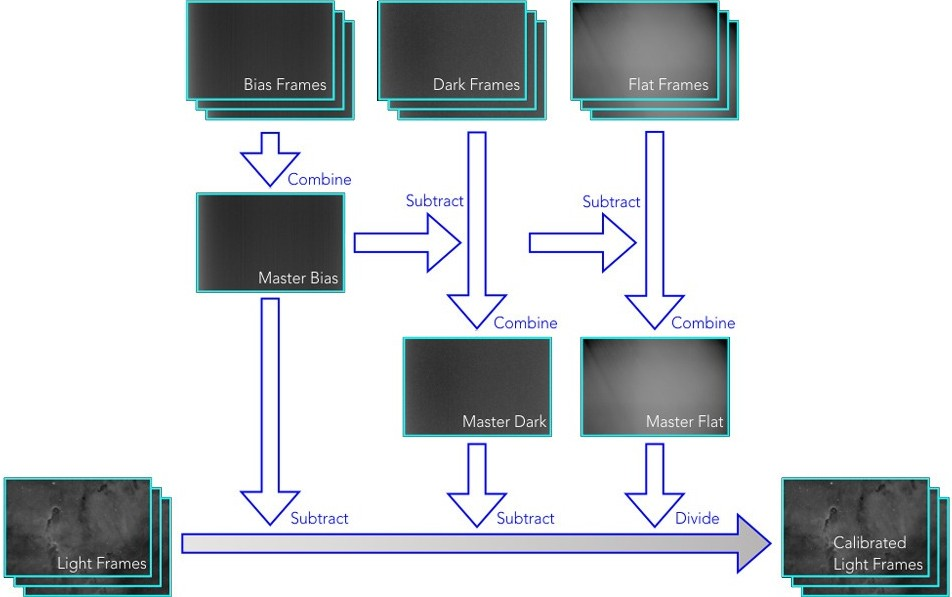
\includegraphics[scale = 0.45]{../assets/calibration_procedure.jpg}
    \captionsetup{justification=centering}
    \caption{Illustrazione schematica dell'uso di immagini di calibrazione \cite{calibration_img}} \label{fig:calibration}
\end{figure}

\section{Allineamento delle immagini} \label{sec:alignment}

L'allineamento delle immagini è un passaggio cruciale nell'elaborazione delle immagini lunari, necessario per compensare eventuali spostamenti o rotazioni tra gli scatti e per combinare efficacemente più immagini tramite tecniche di \textit{stacking}. Questo processo si basa sull'identificazione di punti caratteristici comuni tra le immagini e sul calcolo delle trasformazioni geometriche necessarie (nel nostro caso \hyperref[subsec:homography]{trasformazioni omografiche}) per sovrapporle perfettamente. L'allineamento delle immagini può essere eseguito manualmente, ma è preferibile utilizzare algoritmi automatici per garantire una maggiore precisione e riproducibilità.

\subsection{Feature Detection e Matching ORB, SIFT e SURF} \label{subsec:feature_detection}

Gli algoritmi di \textit{feature detection} e \textit{matching} individuano punti di interesse nei distintivi nelle immagini, come bordi, angoli o altre caratteristiche uniche, e calcolando descrittori che rappresentano l'intensità locale attorno a ciascun punto. Successivamente, i descrittori vengono confrontati per trovare corrispondenze tra i punti di interesse delle diverse immagini, consentendo di determinare le trasformazioni geometriche necessarie per allineare le immagini.

Tra i vari algoritmi di feature detection e matching disponibili, tre si distinguono per la loro efficacia e diffusione: ORB (Oriented FAST and Rotated BRIEF), SIFT (Scale-Invariant Feature Transform) e SURF (Speeded-Up Robust Features), i quali sono in grado di identificare punti di interesse invarianti rispetto a rotazioni, traslazioni e scalature, e sono particolarmente adatti per l'allineamento di immagini astronomiche.

\begin{itemize}
    \item \textbf{SIFT} (Scale-Invariant Feature Transform): è noto per la sua elevata accuratezza e robustezza a cambiamenti di scala, rotazione e illuminazione. L'algoritmo identifica i keypoints costruendo una piramide di immagini a diverse scale e cercando i massimi locali. L'orientamento di ogni keypoint viene determinato analizzando gli istogrammi dell'orientamento del gradiente nell'intorno del punto stesso. Un descrittore SIFT ha generalmente 128 dimensioni e viene calcolato campionando gli orientamenti del gradiente in una griglia 16x16 attorno al punto chiave. Questo algoritmo è molto preciso, ma anche computazionalmente costoso, il che può essere problematico per applicazioni in tempo reale o con grandi volumi di dati \cite{sift}.
    
    \item \textbf{SURF} (Speeded-Up Robust Features): è stato sviluppato come alternativa più veloce a SIFT. Utilizza un'approssimazione del determinante dell'Hessiana per il rilevamento di keypoints e un descrittore basato sulla somma delle risposte alle wavelet di Haar. Questo approccio rende SURF più efficiente dal punto di vista computazionale rispetto a SIFT, pur mantenendo un buon livello di accuratezza e robustezza. Inoltre, SURF integra le informazioni sul gradiente all'interno di un sotto-patch, migliorando le performance nella rilevazione di caratteristiche in presenza di rumore. Tuttavia, come SIFT, anche SURF è coperto da brevetti che ne limitano l'utilizzo \cite{surf}.

    \item \textbf{ORB} (Oriented FAST and Rotated BRIEF): è un descrittore binario veloce, progettato per essere efficiente dal punto di vista computazionale e libero da restrizioni di licenza. Combina il rilevatore di keypoints FAST, noto per la sua rapidità, con un descrittore BRIEF ruotato, che è efficiente da calcolare e confrontare. ORB aggiunge un componente di orientamento veloce e accurato a FAST, consentendo di calcolare in modo efficiente le caratteristiche BRIEF orientate. Per migliorare le prestazioni, ORB utilizza un metodo di apprendimento per decorrelare le caratteristiche BRIEF, garantendo invarianza rotazionale. Rispetto ad algoritmi come SIFT e SURF, ORB offre prestazioni comparabili in molte situazioni, pur essendo significativamente più veloce; dimostra una notevole resistenza al rumore gaussiano, anche se, in presenza di forti distorsioni prospettiche, può risultare meno preciso \cite{orb}.
 
\end{itemize}

Nel contestro di questo progetto, è stato scelto di utilizzare l'algoritmo ORB grazie alla sua efficienza computazionale e alla sua robustezza nei confronti di rotazioni e traslazioni, comuni nelle immagini acquisite senza montature motorizzate. Tuttavia l'implementazione prevede la possibilità di utilizzare anche SIFT e SURF, mediante un'interfaccia comune per la selezione dell'algoritmo di feature detection e matching.

\begin{figure} [H]
    \centering
    \includegraphics[scale = 0.32]{../assets/feature_detection_1.jpg}
    \captionsetup{format=plain}
    \caption{\parbox{0.8\linewidth}{
        Applicazione di ORB (\textbf{a}-\textbf{b}) e RANSAC (\textbf{c}) su due scatti da me acquisiti. \\ \phantom{m}\textbf{a}-\textbf{b}: visualizzazione di 5000 \textit{keypoint} estratti da due immagini} \\ \phantom{MMmnnnc} \textbf{c}: visualizzazione dei \textit{matches} tra i keypoints delle due immagini
    } \label{fig:orb_img}
\end{figure}

\subsection{Trasformazioni omografiche: RANSAC} \label{subsec:homography}

Una \textbf{omografia} è una trasformazione geometrica che mappa punti da un piano a un altro, mantenendo la collinearità e la connessività dei punti. Nel contesto dell'allineamento delle immagini, l'omografia viene utilizzata per correggere le  differenze di posizione, scala, rotazione e prospettiva tra le immagini.

L'omografia è rappresentata da una matrice $3\times3$ denotata con \textbf{H} che descrive una trasformazione tra due piani proiettivi. La relazione tra un punto nell'immagine di origine $(x, y)$ e il suo corrispondente nell'immagine trasformata $(x', y')$ è data dalla seguente equazione:

$$
\begin{bmatrix} x' \\ y' \\ \omega' \end{bmatrix} = H \cdot \begin{bmatrix} x \\ y \\ \omega \end{bmatrix}
$$

dove $\omega$ e $\omega'$ sono i fattori di scala che consentono di rappresentare le trasformazioni proiettive e le coordinate finali sono ottenute dividendo per $\omega'$:

$$
\begin{bmatrix} x'' \\ y'' \end{bmatrix} = \begin{bmatrix} {x'}/{w'} \\ \dfrac {y'} {w'} \end{bmatrix}
$$

L'omografia può essere calcolata a partire da un set di corrispondenze tra punti nelle due immagini, utilizzando l'algoritmo \textbf{RANSAC} (Random Sample Consensus) per stimare i parametri della matrice H.

$$
H = \begin{bmatrix} h_{11} & h_{12} & h_{13} \\ h_{21} & h_{22} & h_{23} \\ h_{31} & h_{32} & h_{33} \ \end{bmatrix}
$$

L'idea alla base di RANSAC è che gli \textit{inlier} (le corrispondenze corrette) concordano tra loro sulla trasformazione da stimare, mentre gli \textit{outlier} (le corrispondenze errate) non concordano e tendono a essere incoerenti \cite{ransac}. 

\begin{enumerate}
    \item Seleziona casualmente un sottoinsieme minimo di corrispondenze. 
    \item Stima il modello (in questo caso, l'omografia) usando il sottoinsieme selezionato.
    \item Calcola un errore di adattamento per tutte le corrispondenze. 
    \item Determina gli inliers come le corrispondenze con errore inferiore a una soglia.
    \item Se il numero di inlier è superiore a una soglia, ricalcola il modello usando tutti gli inlier e termina. 
    \item Altrimenti, ripete i passaggi precedenti per un numero prefissato di iterazioni. 
\end{enumerate}

RANSAC dipende da due parametri: il \textit{numero di iterazioni} e la \textit{soglia di errore}. Un numero maggiore di iterazioni determina quante volte l'algoritmo estrae campioni casuali. Deve essere sufficientemente grande per garantire una probabilità alta di trovare un modello senza outlier. La soglia di errore definisce il massimo errore accettabile per considerare una corrispondenza come inlier. Esistono altri parametri, uno dei quali è il \textit{numero di corrispondenze} da selezionare per stimare l'omografia, solitamente 4. Qui sotto è riportato un esempio di pseudocodice per il calcolo dell'omografia tramite RANSAC.

\begin{algorithm}[H]
    \caption{\texttt{- Algoritmo RANSAC per la stima dell'omografia}:\\ Dati $matches$, la lista di matches, $k$, il numero massimo di iterazioni, $thr$, la soglia per determinare gli inlier e $n$, il numero di corrispondenze da selezionare per l'omografia, l'algoritmo ritorna la matrice omografica stimata.} \label{alg:ransac}
    \begin{algorithmic}[1]
        \Function{estimate\_homography}{$matches, k, thr$}
            \State $H^* \gets$ \textit{null} \Comment{Miglior omografia stimata}
            \State $score^* \gets 0$ \Comment{Miglior punteggio}
            \For{$i \gets 1$ to $k$}
                \State $R \subseteq matches$ con $|R| = n$ \Comment{Seleziona $n$ corrispondenze casuali}
                \State $H \gets$ Stima l'omografia usando $R$
                \State $score \gets 0$
                \For{$m \in matches$}
                    \If{errore($H$, $m$) $< thr$} \Comment{Errore come distanza euclidea}
                        \State $score \gets score + 1$ \Comment{Conta gli   inlier}
                    \EndIf
                \EndFor
                \If{$score > score^*$} \Comment{Seleziona il modello migliore}
                    \State Aggiorna $H^*$ e $score^*$
                \EndIf
            \EndFor
            \State \textbf{return} $H^*$
        \EndFunction
    \end{algorithmic}
\end{algorithm}

Il numero di iterazioni $k$ necessarie per garantire una certa probabilità di successo $P$ dipende dalla percentuale di inlier attesa $p$ e dal numero minimo di punti $n$ richiesti per stimare il modello \cite{ransac_analysis}:

$$
k = \dfrac{\log(1 - P)}{\log(1 - p^n)}
$$

Ad esempio, se si prevede che l'$80\%$ delle corrispondenze siano inlier ($p=0,8$), si desidera una probabilità di successo del $99\%$ ($P=0,99$) e si utilizzano $n=4$ punti per stimare l'omografia, il numero di iterazioni necessarie è:

$$
k = \dfrac{\log(1 - 0.99)}{\log(1 - 0.8^4)} \approx 17.6
$$

\subsection{Algoritmo di allineamento completo} \label{subsec:alignment_complete}

Per ottenere un allineamento più preciso delle immagini, spesso si applica una fase di pre-elaborazione volta a evidenziare le caratteristiche significative. In particolare, i fotogrammi destinati all’estrazione delle caratteristiche vengono convertiti in scala di grigi e sottoposti a filtri per migliorarne nitidezza e contrasto. È importante sottolineare che queste operazioni vengono eseguite su una copia dei fotogrammi, utilizzata esclusivamente per l’estrazione delle caratteristiche, preservando così i dati originali. In questa sezione, tali operazioni sono sintetizzate nella funzione \texttt{enhance()}, (più nel dettaglio nella \cref{subsec:alignment_impl}). 

L'algoritmo completo per l'allineamento delle immagini, che combina le fasi di estrazione delle caratteristiche, corrispondenza dei descrittori, stima dell'omografia tramite RANSAC e applicazione della trasformazione alle immagini, è illustrato nell'\cref{alg:align}.

\begin{algorithm}[H] \caption{\texttt{Allineamento delle immagini}:\\ Data un insieme di immagini $I$, restituisce l'insieme di immagini allineate $A$} \label{alg:align}
    \begin{algorithmic}[1]
        \Function{align\_images}{$I$}
            \State Seleziona un riferimento $r$ \Comment{Tipicamente la più nitida}
            \State $f \gets$ un algoritmo tra ORB, SIFT, SURF
            \State $k_{r}, d_{r} \gets$ f.calculate\_descriptors($r$) \Comment{Calcola keypoints e descrittori di $r$}
            \For{ogni $i$ in $I$}
                \State $k, d \gets$ f.calculate\_descriptors($i$) \Comment{Calcola keypoints e descrittori di $i$}
                \State $m \gets$ match\_descriptors($d_{r}, d$) \Comment{Trova i match tra i descrittori}
                \State $H \gets$ \small ESTIMATE\_HOMOGRAPHY \normalsize ($k_{r}, k, m$) \Comment{Calcola l'omografia}
                \State $a \gets$ apply\_transformation($i$, $H$) \Comment{Applica l'omografia}
                \State Aggiungi $a$ a $A$
            \EndFor
            \State \textbf{return} $A$
        \EndFunction
    \end{algorithmic}
\end{algorithm}

\section{Pre-processing delle immagini} \label{sec:preprocessing}

Il pre-processing delle immagini è quella fase di elaborazione dei singoli scatti (ormai calibrati e allineati), necessaria per migliorare la qualità delle immagini e prepararle per il processo di stacking. Questa fase comprende principalmente il denoising, l'incremento della nitidezza e del contrasto, e l'applicazione di filtri per ridurre l'effetto di \textit{banding} e di \textit{moiré}.

\subsection{Ritaglio delle immagini} \label{subsec:crop}

Nel processo di pre-processing, dopo l'allineamento delle immagini, è utile ritagliare le immagini per focalizzarsi sulla Luna, riducendo la dimensione complessiva dell'immagine. Questo passaggio ha un duplice vantaggio: riduce notevolmente il carico computazionale delle operazioni successive e migliora l'aspetto estetico del risultato finale eliminando porzioni inutili di cielo.

Il processo di ritaglio automatico si basa sull'identificazione del soggetto principale (la Luna) attraverso una sogliatura binaria, seguita dal calcolo di un'area di ritaglio quadrata centrata sul soggetto. L'algoritmo è illustrato in dettaglio nell'\cref{alg:crop}.

\begin{algorithm}[H]
    \caption{\texttt{- Ritaglio automatico delle immagini}:\\ Dato un insieme di immagini allineate $I$ e un margine $m$, l'algoritmo restituisce l'insieme di immagini ritagliate $Out$.} \label{alg:crop}
    \begin{algorithmic}[1]
        \Function{crop\_to\_center}{$I, m$}
            \State $F \gets I[0]$ \Comment{Prima immagine come riferimento}
            \State $G \gets$ Converti $F$ in scala di grigi
            \State $T \gets$ Applica soglia binaria a $G$ \Comment{Separa il soggetto dallo sfondo}
            \State $C \gets$ Trova i contorni in $T$
            \State $B \gets$ Calcola il rettangolo delimitatore del contorno più grande
            \State $x_c, y_c \gets$ Calcola il centro di $B$
            \State $s \gets \max(\text{larghezza}(B), \text{altezza}(B)) + 2m$ \Comment{Dimensione lato}
            \State $x_1 \gets \max\left(x_c - \dfrac{s}{2}, 0\right)$ \Comment{Assicura che sia entro i limiti}
            \State $y_1 \gets \max\left(y_c - \dfrac{s}{2}, 0\right)$
            \State $x_2 \gets \min\left(x_1 + s, \text{larghezza}(F)\right)$
            \State $y_2 \gets \min\left(y_1 + s, \text{altezza}(F)\right)$
            \State $Out \gets []$
            \For{ogni immagine $i$ in $I$}
                \State $c \gets i[y_1:y_2, x_1:x_2]$ \Comment{Ritaglia l'immagine}
                \State Aggiungi $c$ a $Out$
            \EndFor
            \State \textbf{return} $Out$
        \EndFunction
    \end{algorithmic}
\end{algorithm}

È importante notare che, dopo aver calcolato le coordinate di ritaglio $(x_1, y_1)$ e $(x_2, y_2)$, si effettuano controlli per assicurarsi che queste rientrino nei limiti dell'immagine originale, evitando così errori dovuti a coordinate fuori dai bordi.

Per ritagliare un insieme di immagini, si applica la funzione \texttt{crop\_to\_center} con un margine $m$ appropriato. In questo progetto, si è utilizzato un margine compreso tra 10 e 25 pixel, che rappresenta un buon compromesso tra l'inclusione di dettagli periferici e la riduzione di porzioni inutili dell'immagine.

Questa funzione richiede che le immagini siano allineate, poiché le informazioni sul ritaglio vengono calcolate sulla prima immagine, che funge da riferimento, e le altre immagini vengono ritagliate utilizzando le stesse coordinate. Questo assicura che il soggetto principale sia centrato in tutte le immagini ritagliate, facilitando le operazioni successive come lo stacking.

\subsection{Denoising tramite reti neurali: DnCnn} \label{subsec:denoising}

La riduzione del \hyperref[sec:noise]{rumore} (\textit{denoising}) è un passaggio fondamentale per migliorare la qualità delle immagini, specialmente quando si lavora con scatti acquisiti in condizioni non ideali. Nelle immagini lunari, il rumore può nascondere dettagli importanti e compromettere l'efficacia delle tecniche successive, come lo \textit{stacking}.

Tecniche tradizionali di denoising prevedono l'utilizzo di filtri lineari e non, come il filtro gaussiano o il filtro mediano.

\begin{itemize}
    \item \textbf{Filtro mediano}: è un filtro non lineare utilizzato principalmente per ridurre il rumore impulsivo (come il rumore "sale e pepe") in un'immagine. Sostituisce il valore di ogni pixel con la mediana dei valori dei pixel circostanti all'interno di una finestra (o kernel) di dimensione predefinita.
    Dato un'immagine $I(x,y)$ e una finestra di dimensione $m\times m$ centrata sul pixel $(x,y)$, il valore filtrato $I'(x,y)$ è dato da:
    $$
    I'(x,y)=mediana\{I(i,j)|(i,j) \in finestra\}
    $$
    Dove la \textit{mediana} è il valore centrale dei pixel ordinati all'interno della finestra.
    
    \item \textbf{Filtro gaussiano}: è un filtro lineare che applica un'operazione di convoluzione tra l'immagine e una funzione Gaussiana. È utilizzato per ridurre il rumore e sfocare l'immagine, preservando le strutture principali. La funzione Gaussiana bidimensionale con varianza $\sigma^2$ è data da:
    $$
    G_{\sigma}(x,y)=\dfrac{1}{2\pi\sigma^2}\exp{\left(-\dfrac{x^2+y^2}{2\sigma^2}\right)}
    $$
    Il filtro gaussiano applicato all'immagine $I(x,y)$ è definito come:
    $$
    I'(x,y)=\sum_{i=-k}^{k}\sum_{j=-k}^{k}I(x+i,y+j)G(i,j)
    $$
    Dove $k$ è la dimensione del kernel e $\sigma$ controlla l'ampiezza della distribuzione Gaussiana.
    \item \textbf{Filtro bilaterale}: è un'operazione di filtraggio che combina l'informazione spaziale (distanza tra i pixel) e quella radiometrica (differenza di intensità tra i pixel), rendendolo ideale per ridurre il rumore preservando i bordi dell'immagine. La formula generale per il filtro bilaterale è la seguente:
    
    $$
    I'(x,y) = \frac{1}{W(x,y)} \sum_{(i,j) \in S} G_{\sigma_s}\left(\sqrt{(x - i)^2 + (y - j)^2}\right) \, G_{\sigma_r}(I(x,y) - I(i,j)) \, I(i,j)
    $$
    
    Dove $(x,y)$ e $(i,j)$: sono i pixel della finestra locale $S$ in cui viene calcolato il filtro, mentre $I(x,y)$ e $I(i,j)$ sono i valori di intensità rispettivamente del pixel centrale $p$ e del pixel $q$ all'interno della finestra. $W(x,y)$ È il fattore di normalizzazione che assicura che i pesi totali siano normalizzati.
    $$
    W(x,y) = \sum_{(i,j) \in S} G_{\sigma_s}\left(\sqrt{(x - i)^2 + (y - j)^2}\right) G_{\sigma_r}(I(x,y) - I(i,j))
    $$

    Il filtro bilaterale è computazionalmente costoso, poiché richiede il calcolo di due funzioni Gaussiane per ogni pixel dell'immagine.
    
\end{itemize}

Questi filtri riducono il rumore, ma tendono a sfocare l'immagine e a ridurre la nitidezza dei dettagli. Per superare questo problema, negli ultimi anni sono state sviluppate tecniche di denoising basate su reti neurali, che sfruttano la capacità delle reti di apprendere modelli complessi e non lineari direttamente dai dati.

In questo progetto è stato utilizzato \textbf{DnCNN} (Denoising Convolutional Neural Network), una rete neurale profonda progettata specificamente per il denoising di immagini. DnCNN è composto da 17 strati convoluzionali, seguiti da funzioni di attivazione ReLU e da un layer di regressione:

\begin{itemize}
    \item \textbf{Strato di input}: accetta l'immagine rumorosa normalizzata.
    \item \textbf{Strato convoluzionale iniziale}: un layer convoluzionale con 64 filtri $3 \times 3$, padding di 1 pixel, seguito da una funzione di attivazione ReLU. \item \textbf{Strati convoluzionali intermedi}: 15 strati convoluzionali con 64 filtri $3 \times 3$, padding di 1 pixel, ciascuno seguito da \textit{batch normalization} e funzione di attivazione ReLU. \item \textbf{Strato convoluzionale finale}: un layer convoluzionale con un filtro $3 \times 3$, padding di 1 pixel, che fornisce l'output. 
    \item \textbf{Strato di output}: fornisce una stima del rumore presente nell'immagine.
\end{itemize}

\begin{figure}[H]
    \centering
    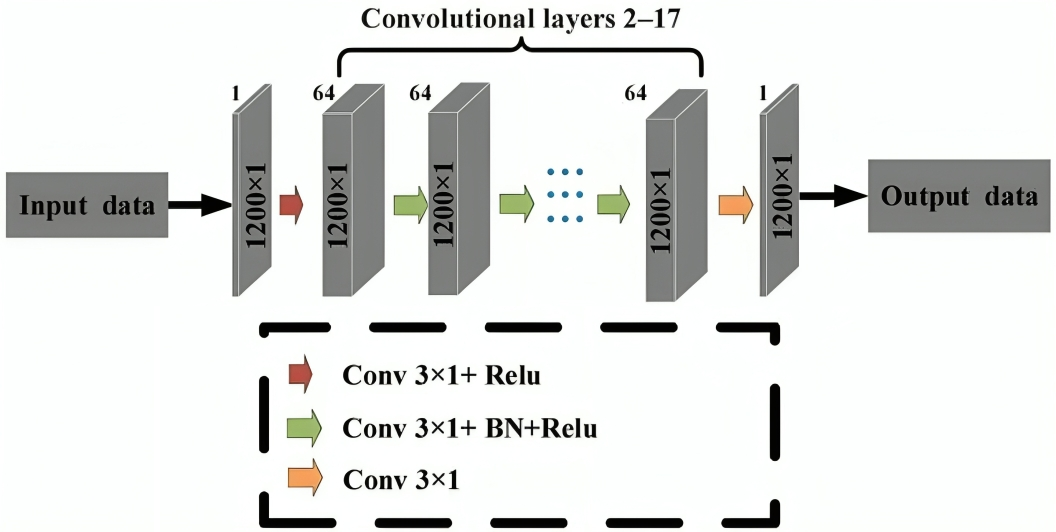
\includegraphics[scale=0.3]{../assets/dncnn.png}
    \captionsetup{justification=centering}
    \caption{Architettura di DnCNN \cite{dncnn_img}} \label{fig:dncnn}
\end{figure}

La rete è addestrata per apprendere la mappatura residua $R(I) = I - I_{\text{denoised}}$, dove $I$ è l'immagine rumorosa e $I_{\text{denoised}}$ è l'immagine a cui è stato rimosso il rumore. Durante l'inferenza, la nuova immagine si ottiene sottraendo il rumore stimato dall'immagine di input:

$$I_{\text{denoised}} = I - R(I)$$

Un modello pre-addestrato di DnCNN (DnCNN-S-25: con $\sigma$ = 25, e addestrato sul dataset \href{https://github.com/cszn/KAIR}{Train400} di Kai Zhang) è stato utilizzato per ridurre il rumore nelle immagini lunari, migliorando la qualità delle immagini e preparandole per il processo di stacking. La procedura utilizzata per la riduzione del rumore con DnCNN è riportata nell'\cref{alg:dncnn}.

\begin{algorithm}[H]
    \caption{\texttt{- Riduzione del rumore con DnCNN}:\\ Data un'immagine $I$, l'algoritmo restituisce l'immagine denoised $Out$.} \label{alg:dncnn}
    \begin{algorithmic}[1]
        \Function{denoise\_image}{$I$}
            \State $I_n \gets$ Normalizza $I$ tra $0$ e $1$ \Comment{Normalizzazione}
            \State $T \gets$ Converti $I_n$ in tensore
            \State $M \gets$ Carica il modello pre-addestrato DnCNN
            \State $N \gets M(T)$ \Comment{Stima del rumore}
            \State $Out \gets I_n - N$ \Comment{Sottrazione del rumore}
            \State $Out \gets$ Denormalizza $Out$ al range originale
            \State \textbf{return} $Out$
        \EndFunction
    \end{algorithmic}
\end{algorithm}

\subsection{Unsharp Masking e personalizzazione} \label{subsec:unsharp_mask}

L'\textbf{Unsharp Masking} è una tecnica utilizzata per aumentare la nitidezza dei dettagli in un'immagine. Consiste nel sottrarre una versione sfocata dell'immagine originale dall'immagine stessa, enfatizzando i dettagli e i bordi \cite{unsharp_mask_book}. La procedura standard è la seguente:

\begin{algorithm}[H]
    \caption{\texttt{Unsharp Mask}:\\ Data un'immagine $I$, l'algoritmo restituisce l'immagine nitida $Out$.} \label{alg:unsharp}
    \begin{algorithmic}
        \Function {unsharp\_mask}{$I, \alpha$}
            \State $I_{\text{B}} \gets$ Gaussian\_Blur($I$) \Comment{Sfocatura}
            \State $M \gets I - I_{\text{B}}$ \Comment{Calcola la maschera}
            \State $Out \gets I + \alpha \cdot M$ \Comment{Amplifica i dettagli}
            \State \textbf{return} $Out$
        \EndFunction
    \end{algorithmic}
\end{algorithm}


L'Unsharp Masking è un metodo semplice ed efficace per migliorare la nitidezza delle immagini, ma può introdurre artefatti e rumore, specialmente se il fattore di forza $\alpha$ è troppo elevato. Per evitare questi problemi, è possibile personalizzare la procedura di Unsharp Masking, ad esempio applicando un filtro di sfocatura diverso, regolando il fattore di forza o utilizzando tecniche di \textit{edge-aware filtering} per preservare i dettagli \cite{unsharp_mask}.

In questo progetto è stata implementata una versione personalizzata dell'unsharp masking che combina la riduzione del rumore tramite DnCNN e l'uso di una maschera basata sul gradiente dell'immagine.

L'applicazione di DnCNN alle immaginni lunari ha portato a risultati a prima vista deludenti. Infatti, l'immagine risultante era molto più sfocata rispetto all'originale. Questo è dovuto al fatto che DnCNN è stato addestrato per rimuovere il rumore, ma non per preservare i dettagli. Per ovviare a questo problema, come riportato nell'\cref{alg:custom_unsharp}, è stata utilizzata una maschera basata sul gradiente dell'immagine originale, che enfatizza i dettagli e i bordi in sezioni dell'immagine con valori del gradiente maggiori, mentre applica una riduzione del rumore maggiore nelle zone più uniformi (con valori del gradiente minori).

\begin{algorithm} [H]
    \caption{\texttt{Unsharp Masking personalizzato}:\\ Data un'immagine $I$, un, l'algoritmo restituisce l'immagine nitida $Out$.} \label{alg:custom_unsharp}

    \begin{algorithmic}
        \Function{custom\_unsharp}{$I, \alpha, \beta, thr$}
            \State $I_{\text{D}} \gets$ \Call{denoise\_image}{$I$} \Comment{Riduzione del rumore con l'\cref{alg:dncnn}}
            \State $I_{\text{D}} \gets (I_{\text{D}} \times \alpha) + I \times (1-\alpha)$ \Comment{Attenuazione del denoising}
            \State $G \gets$ Gradient($I$) \Comment{Calcolo del gradiente}
            \State $D_{\text{M}} \gets$ Get\_Mask$(G, thr)$ \Comment{Maschera di denoising}
            \State $D_{\text{M}} \gets$ Gaussian\_Blur$(D_{\text{M}})$ \Comment{Sfoca leggermente la maschera}
            \State $S_{\text{M}} \gets 1-D_{\text{M}}$ \Comment{Maschera di sharpening}
            \State $D \gets (I - I_{\text{D}}) \times \beta$ \Comment{Estrazione dei dettagli}
            \State $Out \gets (I_{\text{D}} \times D_{\text{M}}) + (I + D)\times S_{\text{M}}$ \Comment{Unsharping con dettagli amplificati}
            \State \textbf{return} $Out$
        \EndFunction
    \end{algorithmic}
\end{algorithm}

dove $Get\_Mask(I, thr)$ è una funzione che restituisce una maschera $M$ tale che:

$$
M(i,j) = \begin{cases} 1 & \text{se } G(i,j) < thr \\ 0 & \text{altrimenti} \end{cases}
$$

Il processo consiste dunque in diversi passaggi fondamentali. Si inizia con la riduzione del rumore, applicando il modello DnCNN all'immagine originale per ottenere una versione con rumore ridotto ($I_{\text{D}}$).
Successivamente, si effettua un \textit{blend} delle immagini, combinando l'immagine denoised e quella originale con un fattore $\alpha$, per preservare parte dei dettagli originali.
Il passo successivo prevede il calcolo del gradiente ($G$) dell'immagine originale per individuare le aree con dettagli significativi.
A questo punto, vengono create delle maschere ($D_{\text{M}}$, $S_{\text{M}}$, rispettivamente \textit{Denoise Mask, Sharpen Mask}) basate sul gradiente per distinguere le zone un cui applicare maggior denoising o amplificare i dettagli.
Per l'amplificazione dei dettagli ($D$), si calcola la differenza tra l'immagine originale e quella denoised, amplificandola con un fattore $\beta$ nelle zone con dettagli significativi.
Infine, si combinano le immagini utilizzando le maschere, ottenendo un'immagine finale ($Out$) in cui i dettagli sono stati amplificati e il rumore ridotto.

\subsection{Rimozione dello sfondo}

Se il cielo negli scatti non è perfettamente uniforme, 
potrebbero essere presenti gradienti di luminosità o rumore che influenzano negativamente il processo di stacking. Per ovviare a questo problema, è possibile rimuovere lo sfondo dalle immagini, enfatizzando i dettagli e riducendo l'effetto di gradienti di luminosità.

Una tecnica molto semplice per rimuovere lo sfondo consiste nell'applicare una maschera all'immagine, mantenendo solo i pixel con intensità al di sotto di una soglia specificata. Questo metodo è efficace per rimuovere lo sfondo uniforme, ma potrebbe non funzionare correttamente se il cielo presenta gradienti di luminosità o rumore.

Per superare queste limitazioni, è possibile applicare una trasformazione non lineare all'immagine, che enfatizza i dettagli e riduce il rumore. In questo progetto è stata utilizzata una trasformazione logistica, che comprime i valori dei pixel in un intervallo limitato, enfatizzando i dettagli e riducendo il rumore. L'algoritmo per la rimozione dello sfondo con trasformazione logistica è riportato nell'\cref{alg:remove_background}.

\begin{algorithm}[H]
    \caption{\texttt{- Rimozione dello sfondo}:\\ Data un'immagine $I$ e i parametri $thr$ e $\alpha$, l'algoritmo restituisce l'immagine con lo sfondo rimosso $Out$.} \label{alg:remove_background}
    \begin{algorithmic}[1]
        \Function{remove\_background}{$I, thr, \alpha$}
            \State $M \gets I < thr$ \Comment{Calcola la maschera dello sfondo}
            \State $Out \gets I$
            \For{ogni pixel $p$ in $M$ dove $M[p]=\text{True}$} 
                \State $Out[p] \gets I[p] \times \dfrac{1}{1 + \exp(-\alpha \times (I[p] - thr))}$ \Comment{Trasformazione logistica}
            \EndFor
            \State \textbf{return} $Out$
        \EndFunction
    \end{algorithmic}
\end{algorithm}

\section{Stacking delle immagini} \label{sec:stacking}

Lo \textbf{stacking} è una tecnica fondamentale nell'astrofotografia che consiste nel combinare più immagini dello stesso soggetto per migliorare il rapporto segnale-rumore e rivelare dettagli altrimenti invisibili.

\subsection{Algoritmi di stacking} \label{subsec:stacking}

Questa tecnica sfrutta il fatto che il rumore è un processo stocastico, mentre il segnale è deterministico. Quando si combinano più immagini dello stesso soggetto, il segnale rimane costante, mentre il rumore si riduce proporzionalmente alla radice quadrata del numero di immagini combinate. Questo significa che, se si combinano $N$ immagini, il rapporto segnale-rumore migliora di un fattore $\sqrt{N}$ \cite{stacking}.

Esistono diversi metodi per combinare le immagini durante lo stacking. Nel progetto sono stati implementati quattro metodi di stacking:

\begin{itemize}
    \item \textbf{Mean}: calcola la media pixel per pixel delle immagini. Questo metodo è utile per ridurre il rumore gaussiano e migliorare la qualità dell'immagine finale.
    $$
    I_{stacked} = \dfrac{1}{N} \sum_{i=1}^{N} I_i
    $$
    \item \textbf{Median}: calcola il valore mediano pixel per pixel delle immagini. Questo metodo è utile per ridurre il rumore impulsivo e rimuovere gli outlier.
    $$
    I_{stacked} = \text{median}(I_1, I_2, \ldots, I_N)
    $$
    \item \textbf{Sigma clipping}: calcola la media pixel per pixel delle immagini, escludendo i pixel con valori al di fuori di un intervallo di soglia. Questo metodo è utile per ridurre l'effetto di outlier e artefatti.
    $$
    I_{stacked}(x,y) = \dfrac{1}{N} \sum_{i=1}^{N} I_i(x,y) \quad \text{dove} \quad |I_i(x,y) - \text{mean}(I(x,y))| < k \cdot \sigma(x,y)
    $$
    \item \textbf{Weighted mean}: calcola la media pesata pixel per pixel delle immagini, assegnando pesi diversi in base ad una metrica di qualità, come la nitidezza.
    $$
    I_{stacked} = \dfrac{\sum_{i=1}^{N} W_i \cdot I_i}{\sum_{i=1}^{N} W_i}
    $$
\end{itemize}

L'algoritmo che ha portato a risultati migliori è la media pesata, molto comune in astrofotografia \cite{stacking_algos}, in particolare pesati in base alla nitidezza dell'immagine. L'algoritmo per il calcolo della media pesata è riportato nell'\cref{alg:weighted_mean}.

\begin{algorithm}[H]
    \caption{\texttt{- Stacking con media pesata}:\\ Dato un insieme di immagini $I$ e i pesi $W$, l'algoritmo restituisce l'immagine combinata $Out$.} \label{alg:weighted_mean}
    \begin{algorithmic}[1]
        \Function{weighted\_mean}{$I, W$}
            \State $N \gets$ \text{numero di immagini in } $I$
            \State $H, W_{\text{sum}} \gets 0$
            \For{$i \gets 1$ to $N$}
                \State $H \gets H + W[i] \times I[i]$ \Comment{Somma pesata}
                \State $W_{\text{sum}} \gets W_{\text{sum}} + W[i]$ \Comment{Somma dei pesi}
            \EndFor
            \State $Out \gets H / W_{\text{sum}}$ \Comment{Normalizzazione}
            \State \textbf{return} $Out$
        \EndFunction
    \end{algorithmic}
\end{algorithm}

Questo metodo è particolarmente efficace quando si combinano immagini con differenti livelli di nitidezza, contrasto e rumore, perchè, con una piccola modifica, permette anche di scartare una percentuale di immagini con qualità inferiore, riducendo l'effetto di artefatti e outlier.

\section{Post-Processing delle immagini} \label{sec:postprocessing}

Il post-processing delle immagini è l'ultima fase dell'elaborazione delle immagini lunari, necessaria per migliorare la qualità dell'immagine finale e renderla pronta per l'analisi e la visualizzazione. Questa fase comprende principalmente la regolazione del contrasto e della luminosità, la rimozione di artefatti e la correzione del bilanciamento del colore. 

Questa fase viene generalmente svolta su programmi di editing professionali come photoshop o lightroom, ma è possibile automatizzare il processo utilizzando algoritmi di elaborazione delle immagini.

\subsection{Miglioramento di nitidezza e contrasto} \label{subsec:contrast}

Per quanto riguarda l'aumento della nitidezza, l'\hyperref{unsharp_mask}{Unsharp Masking} (tradizionale) rimane uno dei metodi più efficaci, in quanto enfatizza i dettagli e i bordi dell'immagine. Tuttavia, è importante regolare attentamente i parametri per evitare artefatti e rumore.

L'\textbf{equalizzazione dell'istogramma} è una tecnica che distribuisce uniformemente i valori dei pixel nell'intervallo dinamico dell'immagine, migliorando il contrasto e la luminosità. Tuttavia, l'equalizzaziome standard può amplificare il rumore in aree omogenee e ridurre i dettagli in aree con contrasto già elevato. Inoltre, se l'immagine ha un contrasto limitato, l'equalizzazione dell'istogramma può produrre un'immagine sovraesposta o sottoposta, generando artefatti e perdita di dettagli.

Per superare queste limitazioni, è stata utilizzata la tecnica \textbf{CLACHE} (Contrast Limited Adaptive Histogram Equalization). CLACHE suddivide l'immagine in piccole regioni chiamate \textit{tile} e applica l'equalizzazione dell'istogramma a ciascuna regione separatamente. Inoltre, limita il contrasto di ciascuna regione per evitare l'amplificazione del rumore e la sovraesposizione. L'algoritmo per l'equalizzazione dell'istogramma con CLACHE è riportato nell'\cref{alg:clache}.

\begin{algorithm}[H]
    \caption{\texttt{- Equalizzazione dell'istogramma con CLACHE}:\\ Data un'immagine $I$, l'algoritmo restituisce l'immagine equalizzata $Out$.} \label{alg:clache}
    \begin{algorithmic}
        \Function{enhance\_contrast}{$I, \text{clip\_limit}, \text{tile\_grid\_size}$}
            \State $I_{\text{CLAHE}} \gets$ \text{Inizializza un'immagine vuota}
            \State $I_{\text{LAB}} \gets$ Converti $I$ in spazio colore LAB
            \State $L, A, B \gets$ Estrai i canali L, A, B da $I_{\text{LAB}}$
            \State $C \gets$ \text{Inizializza un'oggetto} CLACHE \text{con} tile\_grid\_size \text{e} clip\_limit
            \State $L_{\text{CLAHE}} \gets C.apply\_CLAHE(L)$ \Comment{Applica CLACHE al canale L}
            \State $I_{\text{CLAHE}} \gets$ Combina $L_{\text{CLAHE}}$, $A$ e $B$ in un'immagine
            \State \textbf{return} $I_{\text{CLAHE}}$
        \EndFunction
    \end{algorithmic}
\end{algorithm}

Lo spazio LAB è un modello di colore che separa la luminosità ($L$) dal colore ($A$ e $B$), rendendo più semplice l'applicazione di tecniche di miglioramento del contrasto e della luminosità. L'equalizzazione dell'istogramma viene applicata solo al canale $L$, che rappresenta la luminosità dell'immagine, mentre i canali $A$ e $B$ rimangono inalterati. Questo permette di migliorare il contrasto e la luminosità dell'immagine senza influenzare il colore.

Tramite \texttt{clip\_limit} e \texttt{tile\_grid\_size} è possibile regolare il contrasto e la dimensione delle regioni su cui applicare l'equalizzazione dell'istogramma. Un \texttt{clip\_limit} più alto aumenta il contrasto, mentre un \texttt{tile\_grid\_size} più piccolo permette di equalizzare dettagli più fini.

\subsection{Bilanciamento del colore} \label{subsec:color_balance}

Nel contesto dell'astrofotografia lunare, il bilanciamento del colore è generalmente meno critico rispetto ad altre forme di fotografia, poiché la luna appare prevalentemente in toni di grigio. Tuttavia, può essere utile per correggere tonalità dell'immagine e migliorare la qualità visiva, evidenziando lievi variazioni cromatiche dovute alla composizione minerale sulla superficie. Esistono diversi metodi per il bilanciamento del colore:

\begin{itemize}
    \item \textbf{Correzione automatica del bilanciamento del bianco}: utilizza algoritmi di bilanciamento del bianco automatici per correggere il colore dell'immagine in base alla temperatura del colore. Questo metodo è utile per correggere il colore in modo rapido e semplice.
    \item \textbf{Correzione manuale del bilanciamento del bianco}: permette di regolare manualmente il bilanciamento del bianco dell'immagine, selezionando un punto neutro o una zona grigia come riferimento. Questo metodo è utile per ottenere un controllo preciso sul colore dell'immagine.
    \item \textbf{Correzione del colore selettiva}: permette di regolare selettivamente i toni, la saturazione e la luminosità di specifici colori nell'immagine. Questo metodo è utile per migliorare il colore e il contrasto di parti specifiche dell'immagine.
\end{itemize}

Per questo progetto, è stato adottato un metodo di bilanciamento del colore automatico basato sull'assunzione delle \textbf{Shades of Gray} (tonalità di grigio). Questo approccio presuppone che l'immagine abbia una distribuzione equilibrata delle tonalità di grigio, permettendo di correggere le deviazioni cromatiche tramite la normalizzazione dei canali di colore \cite{shades_of_gray}. I passaggi principali sono i seguenti:

\begin{enumerate}
    \item \textbf{Calcolo della media normalizzata per ciascun canale}: Per ogni canale di colore (RGB), si calcola la media dei valori dei pixel elevati a una potenza specificata ($p$). Questa operazione enfatizza i valori più alti, riducendo l'influenza dei pixel più scuri.
    $$
    S[c] = \left(\dfrac{1}{M \times N} \sum_{x=1}^{M} \sum_{y=1}^{N} I(x,y,c)^{p} \right)^{1/p}
    $$
    \item \textbf{Calcolo della media delle \texttt{norm\_values}}: Si calcola la media delle medie normalizzate ottenute per ciascun canale. Questo valore rappresenta il target di normalizzazione per ogni canale.

    $$
    \mu = \dfrac{1}{3} \sum_{c=1}^{3} S[c]
    $$

    \item \textbf{Calcolo dei fattori di scala}: Per ogni canale, si determina un fattore di scala che normalizza la media del canale rispetto alla media complessiva. Questo assicura che ciascun canale contribuisca equamente alla tonalità di grigio finale.
    
    $$
    f[c] = \dfrac{\mu}{S[c]}
    $$
    
    \item \textbf{Applicazione dei fattori di scala}: Si moltiplicano i valori dei pixel di ogni canale per il rispettivo fattore di scala, correggendo le deviazioni cromatiche.
    
    $$
    Out(x,y,c) = I(x,y,c) \times f[c]
    $$
    
    \item \textbf{Clipping dei valori}: Infine, si assicura che i valori dei pixel rimangano nel range $[0, 1]$ per evitare distorsioni cromatiche.
    
    $$
    Out = \text{clip}(Out, 0, 1)
    $$

\end{enumerate}


Questa tecnica garantisce che l'immagine risultante abbia una distribuzione equilibrata delle tonalità di grigio, correggendo automaticamente le deviazioni cromatiche senza richiedere interventi manuali.
Lo pseudocodice che racchiude questi passaggi è riportato nell'\cref{alg:shades_of_gray}.

\begin{algorithm}[H]
    \caption{\texttt{- Shades of Gray - bilanciamento del colore}:\\ Data un'immagine $I$, l'algoritmo restituisce l'immagine bilanciata $Out$.} \label{alg:shades_of_gray}
    \begin{algorithmic}[1]
        \Function{shades\_of\_gray}{$I, p=6$}
            \State $M, N \gets$ dimensioni di $I$
            \State $S \gets$ inizializza vettore per le norme
            \For{$c \gets 1$ to $3$} \Comment{Per ogni canale RGB}
                \State $S[c] \gets \left(\dfrac{1}{M \times N} \sum_{x=1}^{M} \sum_{y=1}^{N} I(x,y,c)^p \right)^{1/p}$ 
            \EndFor
            \State $\mu \gets \dfrac{1}{3} \sum_{c=1}^{3} S[c]$ \Comment{Media delle norme}
            \For{$c \gets 1$ to $3$}
                \State $f[c] \gets \mu / S[c]$ \Comment{Fattori di scala}
                \For{$x \gets 1$ to $M$}
                    \For{$y \gets 1$ to $N$}
                        \State $Out(x,y,c) \gets I(x,y,c) \times f[c]$ \Comment{Applica bilanciamento}
                    \EndFor
                \EndFor
            \EndFor
            \State $Out \gets \text{clip}(Out, 0, 1)$ \Comment{Limita valori tra 0 e 1}
            \State \textbf{return} $Out$
        \EndFunction
    \end{algorithmic}
\end{algorithm}

\cleardoublepage
\chapter{Implementazione} \label{chap:implementation}

In questo capitolo verrà descritta l'implementazione del software sviluppato per l'elaborazione di immagini lunari. In particolare, verranno presentate le scelte progettuali e le soluzioni adottate per la realizzazione delle funzionalità di calibrazione, allineamento, pre-processing, stacking e post-processing affrontate nel \cref{chap:techniques}. I frammenti di codice riportati in questo capitolo rappresentano solo le parti più significative del software; in molti casi sono state omesse linee di controllo o operazioni di supporto per ragioni di brevità. Per una visione completa si rimanda al repository \href{https://github.com/Spina02/Moon-Stacker.git}{GitHub} del progetto.

\section{Architettura del software} \label{sec:architecture}

Il software è stato sviluppato in linguaggio Python, utilizzando principalmente le librerie OpenCV e NumPy per la manipolazione delle immagini.


\begin{multicols}{2}

    Il progetto segue una struttura modulare, con un file principale \texttt{main.py} che coordina l'esecuzione delle funzioni dei vari moduli. L'inizializzazione delle variabili e dei parametri avviene nel file \texttt{config.py}, che contiene la definizione di alcuni flag (come \texttt{DEBUG}), i percorsi delle cartelle utilizzate (input, output, bias, dark, flat, ecc.) e alcune funzioni per l'inizializzazione delle variabili e delle metriche. La pipeline di elaborazione delle immagini è descritta nel file \texttt{process.py}, che si occupa di chiamare le funzioni di calibrazione (\texttt{calibration.py}), allineamento (\texttt{align.py}), denoising (\texttt{denoise.py}), stacking (\texttt{stacking.py}) e, infine, le operazioni di pre-processing e post-processing (\texttt{enhancement.py}).

    \columnbreak

    \begin{verbatim}
         
        src/
        |-- align.py
        |-- analysis.py
        |-- calibration.py
        |-- config.py
        |-- denoise.py
        |-- enhancement.py
        |-- grid_search.py
        |-- image.py
        |-- main.py
        |-- metrics.py
        |-- model.pth
        |-- process.py
        |-- stacking.py
        `-- utils.py
    \end{verbatim}

\end{multicols}

Il modulo \texttt{utils.py} contiene alcune funzioni di ausiliarie (ad esempio, per creare cartelle di destinazione se non esistenti). All'interno di \texttt{image.py} sono presenti funzioni di utilità per la manipolazione delle immagini, come il caricamento, il salvataggio e la visualizzazione. Inoltre, nel file \texttt{metrics.py} sono presenti funzioni per il calcolo di metriche come il contrasto e la luminosità di un'immagine, e metriche di qualità come \texttt{BRISQUE}, \texttt{NIQE} e \texttt{LIQE}, affrontate più nel dettaglio nel \cref{chap:evaluation}

Nella prossima sezione verrà illustrata la pipeline completa di elaborazione delle immagini.

\section{Pipeline di elaborazione} \label{sec:pipeline_impl}

La pipeline di elaborazione completa è stata implementata nel file \texttt{process.py}. Questo file contiene la funzione \texttt{process\_images}, che esegue l'intera pipeline di elaborazione delle immagini, dalla calibrazione all'allineamento, dallo stacking al post-processing. La funzione prende in input una lista di immagini \texttt{images} e un dizionario di parametri \texttt{params} contenente i parametri di configurazione per la pipeline, e restituisce l'immagine finale elaborata.

\begin{lstlisting}
    def process_images(images=None, params={}):
        det_str    = params.get('det_str',    1.3)
        grad_thr   = params.get('grad_thr',   0.008)
        dns_str    = params.get('dns_str',    1.2)
        stack_alg  = params.get('stack_alg',  'weighted_avg')
        avg_alg    = params.get('avg_alg',    'sharpness')
        ush_str    = params.get('ush_str',    2.35)
        tile_size  = params.get('tile_size',  (19, 19))
        clip_limit = params.get('clip_limit', 0.8)

        # Calibration
        calibrated = calibrate_images(images)

        # Alignment 
        aligned = align_images(images)

        # Pre-processing
        cropped = crop_to_center(aligned)
        denoised = custom_unsharp_mask(aligned, det_str, grad_thr, dns_str)
        no_bg = [soft_threshold(img, 0.05, 50) for img in denoised]

        # Stacking
        stacked = stack_images(no_bg, stack_alg, average_alg)

        # Post-processing
        contrasted = enhance_contrast(stacked, clip_limit, tile_size)
        unsharped = unsharp_mask(contrasted, unsharp_strength)
        final_image = shades_of_gray(unsharped)
        
        return final_image
\end{lstlisting}

I parametri di default sono stati ottenuti eseguendo una grid search (implementata in \texttt{grid\_search.py}) su un paio di set di immagini di test, al fine di trovare i valori ottimali che massimizzano la qualità dell'output finale secondo le metriche implementate in \texttt{metrics.py}. Tale ricerca ha permesso di identificare una configurazione bilanciata di parametri che garantisce risultati accettabili sui diversi set.

Nelle sezioni seguenti verranno illustrate in dettaglio le implementazioni delle singole funzionalità della pipeline, esaminando le scelte progettuali e gli algoritmi utilizzati per ciascun modulo.

\subsection{Calibrazione} \label{subsec:calibration_impl}

La fase di calibrazione è stata implementata nel file \texttt{calibration.py}, dove sono definiti i metodi per calcolare i \textit{master bias}, \textit{dark} e \textit{flat}, e quello per applicare la calibrazione alle immagini.

I metodi per calcolare i master seguono la procedura descritta negli algoritmi \ref{alg:bias}, \ref{alg:dark} e \ref{alg:flat} e sono riportati di seguito:

\begin{lstlisting}
    [label={lst:calculate_masters}]
    # Function to calculate the master bias
    def calculate_master_bias(bias):
        # Calculate the mean
        return np.mean(bias, axis=0)

    # Function to calculate the master dark
    def calculate_master_dark(dark, master_bias=None):
        if master_bias is None: master_bias = np.zeros_like(flat[0])
        # Subtract the master bias, then calculate the mean
        return np.mean(dark - master_bias, axis=0)

    # Function to calculate the master flat
    def calculate_master_flat(flat, master_bias=None, master_dark=None):
        if master_bias is None: master_bias = np.zeros_like(flat[0])
        if master_dark is None: master_dark = np.zeros_like(flat[0])
        # Subtract master bias and dark, then calculate the mean
        master_flat = np.mean(flat-master_bias-master_dark, axis=0)   
        # Normalize the master flat
        mean_flat = np.mean(master_flat)
        if mean_flat != 0: master_flat /= mean_flat
        return master_flat
\end{lstlisting}

Queste funzioni calcolano rispettivamente i master bias, dark e flat, utilizzando la media su tutti i frame di calibrazione disponibili. Se i master bias o dark non sono disponibili, vengono inizializzati a matrici di zeri della stessa dimensione delle immagini di calibrazione. Nel caso di \texttt{calculate\_master\_flat}, dopo aver sottratto il master bias e il master dark, si normalizza il master flat dividendo per la sua media, a condizione che questa sia diversa da zero.

Le funzioni tre funzioni sopra definite vengono chiamate da una funzione ausiliaria (\texttt{calculate\_masters}) che, prima di calcolare i masters, verifica se i frame di calibrazione sono stati caricati correttamente e se hanno le stesse dimensioni delle immagini da calibrare; in caso contrario, viene sollevata un'eccezione. Inoltre, se per un tipo di frames di calibrazione il numero di immagini disponibili è inferiore a una certa soglia \texttt{MIN\_CALIBRATION} specificata nel file di configurazione, il master corrispondente non viene calcolato e viene stampato un messaggio di avviso, poiché con troppi pochi frames il calcolo potrebbe non essere affidabile e introdurre nuovi artefatti.

Questa fase risulta compiutazionalmente onerosa, in quanto richiede il caricamento di tutti i frame di calibrazione in memoria, e il calcolo dei master implica l'elaborazione di ogni singolo pixel di ogni frame. Per questo motivo, è stata implementata la possibilità di salvare i master calcolati su file, in modo da poterli riutilizzare senza doverli ricalcolare ogni volta.

Il metodo per calibrare una singola immagine fa riferimento all'\cref{alg:calibration}. L'implementazione è la seguente:

\begin{lstlisting}
    # Function to calibrate a single image
    def calibrate_single_image(image, master_bias = None, master_dark = None, master_flat = None):
        if master_bias is None and master_dark is None and master_flat is None:
            print("No calibration masters available: skipping")
            return image
        if master_bias is None: master_bias = np.zeros_like(flat[0])
        if master_dark is None: master_dark = np.zeros_like(flat[0])
        if master_flat is None: master_flat = np.ones_like(flat[0])
        # Calibrate the image
        calibrated = (image - master_bias - master_dark)/master_flat
        calibrated = np.clip(calibrated, 0, 1)  # Clip to valid range
        return calibrated
\end{lstlisting}

Nella funzione \texttt{calibrate\_single\_image}, si procede alla calibrazione dell'immagine sottraendo il master bias e il master dark, e dividendo per il master flat. Se uno dei master non è disponibile, viene inizializzato a una matrice di zeri (per bias e dark) o di uni (per flat) della stessa dimensione dell'immagine. In questo modo, sia nel calcolo dei master, sia nella calibrazione di una singola immagine, è possibile non utilizzare uno o più set di frame di calibrazione nel caso in cui non siano disponibili. Infine, si utilizza la funzione \texttt{np.clip} di \texttt{NumPy} per assicurarsi che i valori dell'immagine risultante siano compresi nell'intervallo [0, 1].

\subsection{Allineamento} \label{subsec:alignment_impl}

La fase di allineamento delle immagini è stata implementata nel file \texttt{align.py}. Qui sono definite le funzioni necessarie per allineare le immagini utilizzando algoritmi di \textit{feature detection} e \textit{feature matching} come ORB, SIFT e SURF, e RANSAC per il calcolo della trasformazione omografica, come già affrontato nella \cref{subsec:feature_detection}. L'allineamento è fondamentale per compensare eventuali spostamenti o rotazioni tra gli scatti, garantendo una sovrapposizione precisa delle immagini durante la fase di \textit{stacking}.

Per migliorare i risultati dell'allineamento, le immagini passano prima attraverso una funzione di pre-processing che ne ottimizza la qualità prima dell'estrazione delle feature. Questa funzione è stata implementata nel file \texttt{enhancement.py} e svolge essenzialmente tre compiti:

\begin{enumerate}
    \item \textbf{Convertire la foto in scala di grigi} (se non lo è già): riducendo l'immagine a un solo canale, si alleggerisce il carico computazionale per l'estrazione dei keypoint e dei descrittori, oltre a rendere il processo più robusto a variazioni cromatiche.
    
    \item \textbf{Rimozione dello sfondo}: per facilitare l'estrazione delle features, si è scelto di rimuovere lo sfondo dell'immagine, che potrebbe contenere rumore o dettagli non rilevanti. Questo passaggio è stato implementato tramite la funzione \texttt{soft\_threshold} (\cref{alg:remove_background}), che applica una sogliatura morbida all'immagine, mantenendo solo i pixel con intensità superiore ad una certa soglia \texttt{thr}.
    
    \item \textbf{Miglioramento del contrasto}: questo passaggio, effettuato tramite l'applicazione dell'\cref{alg:clache}, è utile per migliorare la qualità dell'immagine, rendendo più nitidi i dettagli e facilitando l'estrazione delle features.
\end{enumerate}

Inoltre, poiché gli algoritmi di OpenCV richiedono immagini in formato a 8 bit, è stata implementata una funzione \texttt{to\_8bit} che converte l'immagine in un formato a 8 bit, normalizzando i valori dei pixel nell'intervallo [0, 255].

L'implementazione dell'algoritmo è riportata di seguito, mentre le implementazioni di \texttt{soft\_threshold} e \texttt{enhance\_contrast}  sono riportate nella \cref{subsec:preprocessing_impl}.

\begin{lstlisting}[label={lst:pre_align_enhance}]
    def pre_align_enhance(image, clip_limit = 0.8, tile_grid_size = (20,20), thr = 0.05):
        # Convert image to grayscale
        enhanced = image.copy()
        if len(image.shape) == 3:
            enhanced = cv2.cvtColor(enhanced, cv2.COLOR_RGB2GRAY)
        # Remove background using a threshold
        enhanced = soft_threshold(enhanced, thr)
        # Enhance contrast using CLACHE
        enhanced = enhance_contrast(enhanced, clip_limit, tile_grid_size)
        enhanced = to_8bit(enhanced)
        return enhanced
\end{lstlisting}

La funzione principale per l'allineamento è \texttt{align\_images}. Tale funzione prende in input una lista di immagini \texttt{images} e restituisce una lista di immagini allineate \texttt{aligned}. I due parametri opzionali \texttt{method} e \texttt{nfeatures} permettono di specificare l'algoritmo di feature detection da utilizzare (tra \texttt{orb}, \texttt{sift} e \texttt{surf}) e il numero di features da estrarre. I valori di default sono rispettivamente \texttt{orb} e \texttt{5000}.

La funzione \texttt{align\_images} inizialmente crea un oggetto \texttt{detector} e un oggetto \texttt{matcher} in base all'algoritmo scelto per effettuare l'estrazione e il matching delle feature. Inizializza la lista \texttt{aligned\_images} con la prima immagine della lista, che fungerà da immagine di riferimento. Si procede quindi a migliorare quest'ultima tramite la funzione \texttt{pre\_align\_enhance}, sopra riportata. Si estraggono quindi i keypoint e i descrittori dell'immagine di riferimento, che saranno necessari per calcolare l'allineamento di tutte le altre immagini utilizzando la funzione \texttt{align\_image}. Infine, si restituisce la lista di immagini allineate.

L'implementazione è la seguente:

\begin{lstlisting}[label={lst:alignment}]
    def align_images(images, method='orb', nfeatures=5000):
        # Choose the feature detection algorithm
        if method == 'orb':
            detector = cv2.ORB_create(nfeatures=nfeatures)
        elif method == 'sift':
            detector = cv2.SIFT_create(nfeatures=nfeatures)            
        elif method == 'surf':
            detector = cv2.xfeatures2d.SURF_create()
        # Choose the norm for the matcher
        norm = cv2.NORM_HAMMING if method == 'orb' else cv2.NORM_L2
        # Create a matcher object
        matcher = cv2.BFMatcher.create(norm)

        # The first image is the reference image
        ref_image = images[0]
        aligned_images = [ref_image]

        # Enhance the reference image to improve alignment
        enhanced_ref = pre_align_enhance(ref_image)

        # Detect keypoints and descriptors for the reference image
        ref_kp, ref_des = detector.detectAndCompute(enhanced_ref, None)
        ref_shape = (ref_image.shape[1], ref_image.shape[0])

        # Align each image to the reference image
        for idx, image in enumerate(images[1:]):
            aligned_image = align_image(image, enhanced_ref, ref_kp, ref_des, ref_shape, detector, matcher)
            aligned_images.append(aligned_image)

        return aligned_images
\end{lstlisting}

La funzione \texttt{align\_image} funzione prende in input l'immagine da allineare \texttt{image}, i keypoint \texttt{ref\_kp} e i descrittori \texttt{ref\_des} dell'immagine di riferimento, l'oggetto \texttt{detector} e il \texttt{matcher}, e restituisce l'immagine allineata con quella di riferimento.

Per allineare l'immagine, si procede come segue:

\begin{enumerate}
    \item Si applica la funzione \texttt{pre\_align\_enhance} all'immagine da allineare, per migliorarne la qualità.
    \item Si estraggono i keypoints e i descrittori dell'immagine da allineare utilizzando il \texttt{detector} scelto.
    \item Si effettua il matching dei descrittori tra l'immagine di riferimento e quella da allineare.
    \item Si applica il \textit{ratio test} per filtrare i buoni match.
    $$
    \text{matches} = \{m \in \text{matches} \mid m.\text{distance} < 0.75 \cdot n.\text{distance}\}
    $$
    \item Si calcola l'omografia tra i keypoints dell'immagine di riferimento e quelli dell'immagine da allineare. Nel mio caso ho scelto di utilizzare interpolazione \texttt{INTER\_LANCZOS4}, molto utilizzata in astrofotografia per la sua capacità di preservare i dettagli.
    \item Si applica la trasformazione omografica all'immagine da allineare.
\end{enumerate}

L'implementazione di \texttt{align\_image} è riportata qui sotto:

\begin{lstlisting}[label={lst:single_alignment}]
    def align_image(image, ref_kp, ref_des, detector, matcher):
        # Enhance the image for alignment process
        aligned_image = pre_align_enhance(image)

        # Find keypoints and descriptors for the image
        kp, des = detector.detectAndCompute(aligned_image, None)

        # Match the descriptors
        matches = matcher.knnMatch(ref_des, des, k=2)
        
        # Apply the ratio test
        matches = [m for m, n in matches if m.distance < 0.75 * n.distance]
        
        # Compute the homography
        ref_pts = np.float32([ref_kp[m.queryIdx].pt for m in matches]).reshape(-1, 1, 2)
        img_pts = np.float32([kp[m.trainIdx].pt for m in matches]).reshape(-1, 1, 2)
        H, _ = cv2.findHomography(img_pts, ref_pts, cv2.RANSAC, 10.0, maxIters=3000, confidence=0.995)
        shape = image.shape[1], image.shape[0]
        
        # Warp the original image using the final homography
        aligned_image = cv2.warpPerspective(image, H, shape, flags=cv2.INTER_LANCZOS4)
        return aligned_image
\end{lstlisting}

I parametri \texttt{maxIters} e \texttt{confidence} nell'invocazione di \texttt{cv2.findHomography} permettono di regolare il numero massimo di iterazioni e la confidenza richiesta per il calcolo della trasformazione omografica. Questi parametri sono stati scelti in modo da ottenere un buon compromesso tra accuratezza e velocità di esecuzione.

\subsection{Pre-processing} \label{subsec:preprocessing_impl}

La fase di pre-processing affrontata nella \cref{sec:preprocessing} è stata implementata nel file \texttt{enhancement.py}. Questa fase comprende operazioni volte a migliorare la qualità delle immagini calibrate e allineate, preparandole per il processo di stacking. Le operazioni implementate vengono eseguite a cascata e sono:

\begin{itemize}
    \item \textbf{Ritaglio dell immagine} per centrare il soggetto ed eliminare bordi esterni indesiderati
    \item \textbf{Miglioramento della nitidezza} attraverso l'uso di tecniche di Unsharp Mask personalizzate e DnCNN;
    \item \textbf{Rimozione dello sfondo} tramite la sogliatura morbida;
\end{itemize}

Di seguito sono descritte le funzioni implementate per effettuare tali operazioni.

\textbf{Ritaglio dell'immagine}

Il ritaglio dell'immagine, basato sull'\cref{alg:crop}, è stato implementato nella funzione \texttt{crop\_to\_center}. Questa funzione prende in input una lista di immagini allineate \texttt{images} e un margine \texttt{margin} (di default 10 pixel) e restituisce una lista di immagini ritagliate in modo che il soggetto sia centrato e i bordi esterni siano eliminati.

\begin{lstlisting}[label={lst:crop}]
    def crop_to_center(images, margin=10):
    cropped_images = []

    # Process the first image to get the cropping parameters
    ref = images[0]
    gray = ref
    if len(ref.shape) == 3:
        gray = cv2.cvtColor(gray, cv2.COLOR_RGB2GRAY)

    # Binary thresholding
    _, thresh = cv2.threshold(gray, 0.1, 1.0, cv2.THRESH_BINARY)

    # Find contours
    contours, _ = cv2.findContours(to_8bit(thresh), cv2.RETR_EXTERNAL, cv2.CHAIN_APPROX_SIMPLE)
    contour = max(contours, key=cv2.contourArea)

    # Get the bounding rectangle of the selected contour
    x, y, w, h = cv2.boundingRect(contour)
    center_x, center_y = x + w//2, y + h//2 # Calculate the center
    size = max(w, h) + 2 * margin               # Determine the size

    # Calculate the top-left corner of the square
    start_x = max(center_x - size//2, 0)
    start_y = max(center_y - size//2, 0)

    # Ensure the square fits within the image boundaries
    end_x = min(start_x + size, ref.shape[1])
    end_y = min(start_y + size, ref.shape[0])

    # Crop all images using the same parameters
    for image in images:
        cropped_image = image[start_y:end_y, start_x:end_x]
        cropped_image = np.clip(cropped_image, 0, 1)
        cropped_images.append(cropped_image)

    return cropped_images
\end{lstlisting}

Da notare che la funzione \texttt{crop\_to\_center} ritaglia tutte le immagini della lista \texttt{images} utilizzando i parametri di ritaglio calcolati sull'immagine di riferimento. Questo approccio richiede che il soggetto sia centrato in tutte le immagini, altrimenti potrebbero verificarsi problemi di allineamento durante il processo di stacking.

\textbf{Riduzione del rumore e Unsharp Masking con DnCNN}

Come descritto nelle sezioni \ref{subsec:denoising} e \ref{subsec:unsharp_mask}, è stata implementata una versione personalizzata dell'Unsharp Masking che combina la riduzione del rumore tramite DnCNN e l'utilizzo di una maschera basata sul gradiente dell'immagine.

Iniziamo col descrivere l'operazione di denoising con il modello preaddestrato. Per importarlo nel progetto è stato necessario scaricare il modello preaddestrato e salvarlo in un file \texttt{.pth}. Il modello è stato poi caricato utilizzando la libreria \texttt{torch} e la funzione \texttt{torch.load}. Il modello è stato quindi utilizzato per ridurre il rumore delle immagini, come mostrato nel seguente codice.

\begin{lstlisting}[label={lst:dncnn}]
    DNCNN_MODEL_PATH = './src/model.pth'
    
    class DnCNN(nn.Module):
        def __init__(self,depth=17,n_channels=64,image_channels=1):
            super().__init__()
            self.dncnn = nn.Sequential(
                nn.Conv2d(image_channels, n_channels, 3, padding=1), nn.ReLU(inplace=True),
                *[layer_block(n_channels) for _ in range(depth-2)],
                nn.Conv2d(n_channels, image_channels, 3, padding=1)
            )
            self._initialize_weights()
    
        def forward(self, x):
            return x - self.dncnn(x)
    
        def _initialize_weights(self):
            for m in self.modules():
                if isinstance(m, nn.Conv2d):
                    init.orthogonal_(m.weight)
                    if m.bias is not None: init.constant_(m.bias, 0)
                elif isinstance(m, nn.BatchNorm2d):
                    init.constant_(m.weight, 1); init.constant_(m.bias, 0)
    
    def layer_block(n_channels):
        return nn.Sequential(
            nn.Conv2d(n_channels,n_channels,3,padding=1,bias=False),
            nn.BatchNorm2d(n_channels, eps=1e-4, momentum=0.95),
            nn.ReLU(inplace=True)
        )
    
    def model_init(model_path=DNCNN_MODEL_PATH):
        model = torch.load(model_path)
        model.eval()
        return model
\end{lstlisting}

La classe \texttt{DnCNN} implementa una rete neurale convoluzionale profonda progettata specificamente per la riduzione del rumore nelle immagini. Questa rete, denominata \textbf{Denoising Convolutional Neural Network (DnCNN)}, è caratterizzata da una struttura composta da 17 strati convoluzionali, progettati per stimare e rimuovere il rumore presente nell'immagine di input, come visto nella \cref{subsec:denoising}. 

La funzione \texttt{model\_init} si occupa di caricare il modello preaddestrato da un file \texttt{.pth} e restituirlo pronto per l'elaborazione.

Per garantire la compatibilità con il modello DnCNN, le immagini devono essere trasformate in tensori e normalizzate. Dopo il denoising, è necessario riconvertire i tensori in immagini nel formato \texttt{np.float32}. Queste operazioni sono state incapsulate in due funzioni:

\begin{enumerate}
    \item \textbf{\texttt{prepare\_tensor\_for\_model}}: converte un'immagine nel formato tensoriale e la normalizza.

    \item \textbf{\texttt{convert\_tensor\_to\_image}}: riconverte il tensore prodotto dal modello in un'immagine \texttt{np.float32} utilizzabile nei flussi di elaborazione successivi.
\end{enumerate}

L'implementazione di queste funzioni non è riportata per questioni di brevità.

La funzione per effettuare il denoising, basata sull'\cref{alg:dncnn} è quindi la seguente:

\begin{lstlisting}[label={lst:denoise}]
    def perform_denoising(model, image):
        shape = image.shape

        if len(shape) < 3:
            image = cv2.cvtColor(image, cv2.COLOR_GRAY2RGB)
        channels = list(cv2.split(color.rgb2lab(image)))
        
        # convert image to tensor
        l = prepare_tensor_for_model(channels[0], 100).to(device)
        
        if torch.cuda.is_available(): device = torch.device('cuda')
        else: torch.device('cpu')
        model = model.to(device).eval()
        with torch.no_grad():
            denoised_l = model(l).cpu()

        # convert tensor to image
        denoised_l = convert_tensor_to_image(denoised_l, 100)
        channels[0] = denoised_l

        # Merge the channels
        denoised = cv2.merge(channels)
        denoised = color.lab2rgb(denoised)

        if len(shape) < 3:
            denoised = cv2.cvtColor(denoised, cv2.COLOR_RGB2GRAY)

        return denoised
\end{lstlisting}

Come è possibile notare, il denoising viene eseguito solo sul canale L dell'immagine, in quanto è il canale che contiene la maggior parte delle informazioni di luminosità. Dopodiché l'immagine viene riconvertita in RGB e, se necessario, in scala di grigi.

Possiamo ora descrivere l'algoritmo di Unsharp Masking personalizzato, basato sull'\cref{alg:custom_unsharp}, che è stato implementato nella funzione \texttt{custom\_unsharp\_mask}. Questa implementazione combina il denoising tramite DnCNN con una maschera basata sul gradiente dell'immagine per preservare i dettagli importanti.

\begin{lstlisting}[label={lst:unsharp_mask}]
    def custom_unsharp_mask(images, model, det_str=1.3, thr=0.09, dns_str=1.2):
        sharpened_images = []

        for idx, image in enumerate(images):
            # Apply denoising with DnCNN
            denoised = denoise(image, model)
            
            # Blend original and denoised image
            denoised = denoised * dns_str + image * (1 - dns_str)

            # Convert to grayscale for gradient calculation if needed
            gray_image = cv2.cvtColor(image, cv2.COLOR_RGB2GRAY) if image.ndim == 3 else image
            
            # Calculate image gradient magnitude
            grad_mag = np.sqrt(np.gradient(gray)**2, axis=0)

            # Create denoise mask: 1 where gradient is low
            mask = np.where(grad_mag < thr, 1, 0).astype(np.float32)
            # Smooth mask edges
            mask = cv2.GaussianBlur(mask, (3,3), 0.5)

            # Expand mask to 3 channels for RGB images
            if image.ndim == 3:
                mask = np.repeat(mask[:, :, np.newaxis], 3, axis=2)

            # Create detail mask (inverse of denoise mask)
            det_mask = 1 - mask

            # Combine denoised and original image using masks
            final_image = (denoised * mask) + (image * det_mask)

            # Amplify details in high gradient areas
            amplified_details = (image - denoised)@$\,$@*@$\,$@det_str@$\,$@*@$\,$@det_mask
            sharpened_image = final_image + amplified_details

            # Ensure valid pixel range
            sharpened_image = np.clip(sharpened_image, 0, 1)
            sharpened_images.append(sharpened_image)

        return sharpened_images
\end{lstlisting}

La funzione \texttt{custom\_unsharp\_mask} prende in input una lista di immagini \texttt{images}, il modello DnCNN \texttt{model} e i parametri per controllare il processo: \texttt{det\_str} regola l'intensità dell'amplificazione dei dettagli, \texttt{thr} definisce la soglia per distinguere aree di dettaglio da aree uniformi e \texttt{dns\_str} indica l'intensità del denoising sul risultato. 

Per ciascuna immagine, viene applicato il denoising tramite il modello DnCNN, viene poi calcolato il gradiente, da cui si ricavano due maschere che separano zone ad alto dettaglio da quelle più uniformi. La fase finale combina l'immagine originale con quella denoised utilizzando le maschere create, amplificando i dettagli nelle aree ad alto gradiente e privilegiando l'effetto del denoising nelle altre.

\subsection{Stacking} \label{subsec:stacking_impl}

La fase di stacking delle immagini è stata implementata nel file \texttt{stacking.py}. Come descritto nel \cref{sec:stacking}, lo stacking è una tecnica fondamentale in astrofotografia per migliorare il rapporto segnale-rumore combinando più immagini dello stesso soggetto. Nel progetto sono stati implementati tre dei metodi di stacking più comuni:

\begin{itemize}
    \item \textbf{Media Pesata (Weighted Mean)}: calcola la media pesata delle immagini, assegnando pesi basati su una metrica di qualità, come la nitidezza.
    \item \textbf{Mediana (Median Stacking)}: calcola il valore mediano pixel per pixel delle immagini.
    \item \textbf{Sigma Clipping}: calcola la media pixel per pixel escludendo i pixel che deviano oltre una certa soglia dalla media.
\end{itemize}

Il metodo che ha prodotto i risultati migliori è la media pesata, dove i pesi sono determinati in base alla qualità di ciascuna immagine. L'algoritmo è stato implementato nella funzione \texttt{weighted\_average\_stack}.

\begin{lstlisting}[label={lst:weighted_average_stack}]
    def weighted_average_stack(images, method='sharpness'):
        # Calculate the weights for each image
        weights = calculate_weights(images, method)
        # Zero out the lowest 10% of the weights
        weights[np.argsort(weights)[:len(weights)//10]] = 0
        weights = weights / np.sum(weights)

        n_ch = 1 if len(images[0].shape) == 2 else images[0].shape[2]
        stacked_channels = []
        for i in range(n_ch):
            # Extract the i-th channel from each image
            channel_stack = np.array([cv2.split(img)[i] for img in images])

            # Calculate the weighted sum of the channels
            stacked_channel = np.zeros_like(channel_stack[0], dtype=np.float64)
            for channel, weight in zip(channel_stack, weights):
                # Weighted sum
                stacked_channel += channel * weight

            stacked_channels.append(stacked_channel)

        # Combine the channels into a single image
        stacked_image = cv2.merge(stacked_channels)
        return stacked_image.astype(np.float32)
\end{lstlisting}

La funzione \texttt{weighted\_average\_stack} calcola i pesi per ciascuna immagine in base alla metrica specificata (chiamando la funzione \texttt{calculate\_weights}), normalizza i pesi e calcola la media pesata dei pixel per ciascun canale. Infine, combina i canali in un'unica immagine.

La metrica che ha portato a risultati migliori è stata la nitidezza, ma è possibile utilizzare anche altre metriche.

La funzione \texttt{calculate\_weights} per calcolare i pesi è riportata di seguito:

\begin{lstlisting}[label={lst:calculate_weights}]
    def calculate_weights(images, method='sharpness'):
        if method == 'contrast':
            weights = [calculate_contrast(img) for img in images]
        elif method == 'sharpness':
            weights = [calculate_sharpness(img) for img in images]
        elif method == 'brisque':
            weights = [1 - normalize(calculate_metric(img, 'brisque_matlab'), 0, 100) for img in images]
        elif method == 'liqe':
            weights = [calculate_metric(img, 'liqe') for img in images]
        else:
            raise ValueError("Unknown method: {}".format(method))
        return weights 
\end{lstlisting}

Le metriche disponibili includono la nitidezza \texttt{sharpness}, il contrasto \texttt{contrast} e le metriche \texttt{BRISQUE} e \texttt{LIQE} di PyIqa. Tutte queste metriche vengono calcolate utilizzando le funzioni definite nel file \texttt{metrics.py}, non riportate per brevità.

Il metodo \texttt{median\_stack} implementa lo stacking per mediana, calcolando il valore mediano pixel per pixel delle immagini. Questo metodo è utile per ridurre l'effetto di outlier e rumore impulsivo.

\begin{lstlisting}[label={lst:median_stack}]
    def median_stack(images):
        n_ch = 1 if len(images[0].shape) == 2 else images[0].shape[2]
        stacked_channels = [np.median([cv2.split(img)[i] for img in images], axis=0) for i in range(n_ch)]
        stacked_image = cv2.merge(stacked_channels)
        return stacked_image.astype(np.float32)
\end{lstlisting}

Il metodo \texttt{sigma\_clipping} implementa lo stacking utilizzando il sigma clipping, che esclude i pixel che deviano oltre una certa soglia (espressa in termini di deviazione standard) dalla media.

\begin{lstlisting}[label={lst:sigma_clipping}]
    def sigma_clipping(images, sigma=3):
        n_ch = 1 if len(images[0].shape) == 2 else images[0].shape[2]
        stacked_channels = []
        for i in range(n_ch):
            channel_stack = np.array([cv2.split(img)[i] for img in images])
            mean = np.mean(channel_stack, axis=0)
            std = np.std(channel_stack, axis=0)
            # Mask for values within @\color{green!40!black} \texttt{sigma $\times$ std}@ from the mean
            mask = np.abs(channel_stack - mean) < sigma * std
            # Clip the values outside the mask to the mean
            clipped = np.where(mask, channel_stack, mean)
            # Calculate the mean of the clipped values
            stacked_channel = np.mean(clipped, axis=0)
            stacked_channels.append(stacked_channel)
        stacked_image = cv2.merge(stacked_channels)
        return stacked_image.astype(np.float32)
\end{lstlisting}

Questo metodo è efficace nel ridurre l'impatto di valori anomali e artefatti.

\subsection{Post-processing} \label{subsec:postprocessing_impl}

La fase di post-processing è stata implementata nel file \texttt{enhancement.py} e comprende diverse operazioni finalizzate a migliorare ulteriormente la qualità dell'immagine dopo lo stacking. Le principali operazioni eseguite sono:

\begin{itemize}
    \item \textbf{Miglioramento della nitidezza} utilizzando l'algoritmo tradizionale di Unsharp Mask.
    \item \textbf{Miglioramento del contrasto} applicando l'algoritmo CLAHE (Contrast Limited Adaptive Histogram Equalization).
    \item \textbf{Bilanciamento del colore} per correggere eventuali dominanti cromatiche presenti nell'immagine finale.
\end{itemize}

Di seguito sono descritte le implementazioni di queste operazioni.

\textbf{Miglioramento della nitidezza con Unsharp Mask}

Dopo lo stacking, può essere utile aumentare ulteriormente la nitidezza dell'immagine per enfatizzare i dettagli superficiali della Luna. L'algoritmo di Unsharp Mask tradizionale è stato utilizzato per questo scopo, implementato nella funzione \texttt{unsharp\_mask}.

\begin{lstlisting}[label={lst:unsharp_mask}]
    def unsharp_mask(image, strength):
        # Apply a Gaussian filter to blur the image
        blurred_image = cv2.GaussianBlur(image, (3, 3), 0.5)

        # Combine the blurred image with the original image
        sharpened_image = cv2.addWeighted(image, 1 + strength, blurred_image, -strength, 0)

        # Clip the values to the valid range
        sharpened_image = np.clip(sharpened_image, 0, 1)

        return sharpened_image
\end{lstlisting}

In questa funzione, viene applicato un filtro Gaussiano per ottenere una versione sfocata dell'immagine. La differenza tra l'immagine originale e quella sfocata viene poi amplificata di un fattore \texttt{strength} e sommata all'originale. Questo approccio, descritto in dettaglio nella \cref{subsec:unsharp_mask}, incrementa efficacemente la nitidezza dell'immagine preservando al contempo la naturalezza dei dettagli e minimizzando l'introduzione di artefatti.

Il parametro \texttt{strength} consente un controllo preciso sull'intensità dell'effetto di sharpening. Attraverso test empirici condotti nell'ambito di questo progetto, è stato determinato che valori intorno a 2.35 forniscono il miglior compromesso tra miglioramento della nitidezza e preservazione della qualità dell'immagine.

\textbf{Miglioramento del contrasto con CLAHE}

Per migliorare il contrasto locale e rendere più visibili le variazioni tonali nell'immagine, è stato utilizzato l'algoritmo CLAHE (Contrast Limited Adaptive Histogram Equalization), descritto nell'\cref{alg:clache}.

L'implementazione è stata realizzata nella funzione \texttt{enhance\_contrast}.

\begin{lstlisting}[label={lst:clache}]
    def enhance_contrast(image, clip_limit = 0.07, tile_size = (20, 20)):
        if len(image.shape) < 3: image = cv2.cvtColor(image, cv2.COLOR_GRAY2RGB)

        # Convert the image to LAB color space
        lab = cv2.cvtColor(image, cv2.COLOR_RGB2LAB)
        l_channel = lab[:, :, 0]

        # Apply CLAHE to the L channel
        clahe = cv2.createCLAHE(clipLimit=clip_limit, tileGridSize=tile_size)
        l_channel_equalized = clahe.apply(l_channel)

        # Update the L channel
        lab[:, :, 0] = l_channel_equalized

        # Convert the image back to RGB color space
        enhanced_image = cv2.cvtColor(lab, cv2.COLOR_LAB2RGB)

        return enhanced_image
\end{lstlisting}

L'algoritmo migliora il contrasto locale dell'immagine, rendendo più evidenti i dettagli nelle aree scure o chiare. I parametri \texttt{clip\_limit} e \texttt{tile\_grid\_size} permettono di regolare il livello di contrasto e la dimensione dei blocchi utilizzati per il calcolo dell'istogramma. I valori di default sono stati scelti in modo da ottenere risultati ottimali.

\textbf{Bilanciamento del colore}

Per correggere eventuali dominanti cromatiche e bilanciare i colori dell'immagine finale, è stato applicato nuovamente l'algoritmo \texttt{Shades of Gray}, già descritto nella \cref{subsec:color_balance}. L'implementazione è la seguente:

\begin{lstlisting}[label={lst:color_balance}]
    def shades_of_gray(image, power=6):
        # Calculate norm values for each channel using Minkowski norm
        norm_values = np.power(np.mean(np.power(image, power), axis=(0, 1)), 1 / power)
        
        # Calculate the mean of the norm values
        mean_norm = np.mean(norm_values)
        
        # Calculate scaling factors to balance the color channels
        scale_factors = mean_norm / norm_values
        
        # Apply the scaling factors to balance the image
        balanced_image = image * scale_factors
        
        # Clip values to valid range [0,1]
        balanced_image = np.clip(balanced_image, 0, 1)

        return balanced_image 
\end{lstlisting}

Questa funzione normalizza i canali di colore dell'immagine, correggendo le deviazioni cromatiche e garantendo una resa cromatica più naturale.

Le operazioni di post-processing vengono eseguite in sequenza per ottenere un'immagine finale ottimizzata. Dopo lo stacking, l'immagine passa attraverso l'Unsharp Mask per migliorare la nitidezza, CLAHE per aumentare il contrasto e infine Shades of Gray per bilanciare i colori. Questa sequenza garantisce che i dettagli siano ben definiti, il contrasto elevato e i colori equilibrati, migliorando significativamente la qualità visiva dell'immagine finale.

Per assicurare che le operazioni di post-processing funzionino correttamente indipendentemente dalle condizioni iniziali dell'immagine, è stata implementata una gestione delle immagini in scala di grigi e a colori. Ad esempio, se l'immagine è in scala di grigi, viene convertita temporaneamente in formato RGB prima di applicare CLAHE, per evitare errori di dimensionamento dei canali.

\section{Sfide affrontate e soluzioni adottate} \label{sec:challenges}

Durante la fase di progettazione e implementazione del progetto, sono state affrontate diverse sfide. Alcune di esse sono state risolte, mentre altre, a causa di limitazioni di tempo o risorse, rimangono aperte per futuri sviluppi.

\subsection{Alto utilizzo di RAM}

Un problema significativo riscontrato durante lo sviluppo è stato l'elevato utilizzo di memoria RAM da parte del programma. Tale problema è stato causato principalmente dall'uso di numerose immagini ad medio-alta risoluzione, che richiedono molta memoria per essere elaborate. La causa principale risiede nell'implementazione della funzione per la lettura e il caricamento delle immagini in memoria. Questo metodo prende in input il percorso della cartella contenente le foto e le apre tutte contemporaneamente (utilizzando metodi diversi in base al formato), inserendole in una lista.

\begin{lstlisting}[label={lst:read_images}]
    def read_image(file_path):
        if file_path.lower().endswith(('.tiff', '.tif')):
            return imageio.imread(file_path).astype(np.float32)
        if file_path.lower().endswith(raw_formats):
            with rawpy.imread(file_path) as raw:
                # convert to rgb image using the camera white balance
                return to_float32(raw.postprocess(use_camera_wb=True, no_auto_bright=True, output_bps=16))
        else:
            return to_float32(imageio.imread(file_path))

    def read_images(folder_path, max_img=MAX_IMG):
        img_paths = read_folder(folder_path, max_img)
        @\color{red}\textit{\# $\ ------ \downarrow$ here is where the problem lies $\downarrow ------$}@
        images = [read_image(path) for path in img_paths]
\end{lstlisting}

In questo modo, ogni immagine viene caricata in RAM in formato a 32 bit. Lavorando con insiemi di 20-30 di immagini l'uno (ad esempio nella fase di calibrazione sono stati utilizzati 30 bias frames e altrettanti dark frames, per un totale di circa 90 immagini caricate in memoria contemporaneamente) spesso il programma termina in modo anomalo a causa dell'uso eccessivo di memoria. Per ovviare a questo problema, è stata suddivisa la pipeline in stadi intermedi nei quali vengono salvati i risultati parziali in formato TIFF a 32 bit. In questo modo, è possibile riavviare l'esecuzione del programma senza dover ricalcolare tutti gli step precedenti al crash; tuttavia questa non rappresenta una soluzione ottimale.

Una soluzione più adatta a questo problema è quella dell'uso di generatori per leggere le immagini. Ciò permette di caricare in memoria solo un'immagine alla volta, riducendo notevolmente l'uso di RAM. Una possibile implementazione è la seguente:

\begin{lstlisting}[label={lst:image_generator}]
    def read_images_generator(folder_path, max_imgs=None):
        loaded = 0
        for filename in sorted(os.listdir(folder_path)):
            if max_imgs is not None and loaded >= max_imgs:
                break
            img_path = os.path.join(folder_path, filename)
            if os.path.isfile(img_path):
                if img_path.lower().endswith(('.tiff', '.tif')):
                    yield imageio.imread(img_path).astype(np.float32)
                if img_path.lower().endswith(raw_formats):
                    with rawpy.imread(img_path) as raw:
                        # convert to rgb image using the camera wb
                        yield to_float32(raw.postprocess(use_camera_wb=True, no_auto_bright=True, output_bps=16))
                else:
                    yield to_float32(imageio.imread(img_path))
                loaded += 1
\end{lstlisting}

Questo metodo è stato testato per generare le immagini di analisi e ha portato a un notevole risparmio di memoria. Si propone quindi come soluzione per futuri sviluppi.

L'utilizzo intensivo di memoria ha spesso influenzato le scelte di progetto, portando a preferire soluzioni più efficienti dal punto di vista della memoria, anche a discapito della velocità di esecuzione. Un esempio si ha nella scelta dell'immagine di riferimento per l'allineamento; inizialmente si era pensato di selezionare tra le immagini acquisite quella con la migliore qualità, ma ciò avrebbe richiesto il caricamento in memoria di tutte le immagini per confrontarle, con un conseguente aumento dell'uso di RAM. Si è quindi preferito utilizzare la prima immagine come riferimento, anche se ciò potrebbe portare a risultati di allineamento meno precisi nel caso in cui la qualità dell'immagine di riferimento fosse inferiore rispetto alle altre.

\subsection{Ricerca dei parametri ottimali}

Una delle maggiori sfide di questo progetto è stata la ricerca dei parametri ottimali per l'elaborazione delle immagini. Molti parametri dipendono fortemente dalle immagini in ingresso, come la soglia \texttt{grad\_thr} per generare la maschera dal gradiente, o \texttt{dns\_str}, che regola l'intensità del denoising da applicare alla foto, entrambi nella funzione \texttt{custom\_unsharp\_mask}. È quindi necessario effettuare una ricerca avanzata dei parametri per rendere i risultati ottimali indipendentemente da fattori come la luminosità, il contrasto e la quantità di rumore, presenti nelle immagini di partenza. 

Un'alternativa per ottenere risultati più precisi consiste nell'estrarre i valori di tali parametri direttamente dalle caratteristiche delle immagini di partenza. Ad esempio, il parametro \texttt{tile\_size} dipende principalmente dalle dimensioni dell'immagine, più che da caratteristiche della foto in sé; dopo diverse prove, è stato notato che si ottengono risultati migliori per valori che si aggirano attorno a 1/70 delle dimensioni dell'immagine dopo la fase di ritaglio.

Un ulteriore problema riguarda la valutazione dei risultati nella ricerca dei parametri. Quando si ha a che fare anche solo con una decina di parametri da testare, provando tre valori per ciascuno di essi, si ottengono migliaia di foto in output, rendendo l'analisi visiva impossibile. Inoltre, spesso si osservano variazioni tra le immagini non sempre distinguibili ad occhio nudo. È quindi necessario stabilire una metrica di riferimento che rifletta il miglioramento visivo dell'immagine. Da ciò sorge un ulteriore problema: l'assenza di un'immagine di riferimento.

\subsection{Assenza di immagine di riferimento}

Come verrà illustrato nel \cref{chap:evaluation}, la metrica di valutazione maggiormente adottata nel contesto dell'astrofotografia è il rapporto segnale-rumore (SNR). Questa metrica, per essere calcolata, richiede la presenza di un'immagine di riferimento ideale a cui il programma deve tendere. Poiché le immagini sono state acquisite durante il progetto, non era disponibile un'immagine di riferimento ideale. È stato quindi tentato di utilizzare come riferimento un'immagine (scaricabile dai siti INAF o NASA) acquisita dal Lunar Reconnaissance Orbiter (LRO), un satellite in orbita intorno alla Luna. Questo satellite ha compiuto diversi scatti, da cui è stata elaborata l’immagine finale tramite la tecnica dello stitching. Tuttavia, ciò causa problemi di compatibilità con le immagini acquisite. Infatti, la foto di riferimento presenta, nelle aree periferiche della Luna, dettagli che non compaiono nelle immagini acquisite, rendendo impossibile l'allineamento. Sono state inoltre esplorate altre immagini di riferimento, ma quelle ad uso libero trovate su internet spesso non presentano una qualità superiore a quelle utilizzate nel progetto, rendendole quindi inadatte come riferimento “ideale”, oppure sono immagini delle cosiddette "mineral moon", risultanti dalla sovrapposizione di scatti ottenuti attraverso filtri di frequenza, con una colorazione artificiale che le rende non adatte al confronto.

Una tecnica adottata comunemente per risolvere questo problema consiste nel prendere un'immagine di alta qualità e, da essa, generare diversi set di immagini con rumore aggiunto, in modo da simulare le condizioni reali. Questo metodo, chiamato \textit{data augmentation}, è stato adottato in diversi progetti di machine learning e potrebbe essere una soluzione per questo progetto. Tuttavia, vista la mancanza di tempo e di risorse, non è stato possibile implementare questa soluzione, che si rimanda a sviluppi futuri.

Viste le difficoltà affrontate, è stato deciso di utilizzare delle metriche di valutazione senza riferimento, le quali però, come vedremo nel dettaglio nel prossimo capitolo, non sempre sono in grado di percepire il miglioramento effettivo della foto.

\subsection{Pochi dati per testing}

Come già specificato nel capitolo introduttivo, gli scatti sono stati acquisiti tramite una fotocamera bridge Fujifilm Finepix S1, un dispositivo di media gamma, senza l'ausilio di strumentazione professionale come telescopi o montature robotizzate (descritte nella \cref{subsec:hardware}).

Il problema principale è stato rappresentato dalle condizioni meteorologiche, che nei mesi precedenti la realizzazione del progetto sono state raramente favorevoli, permettendo di acquisire pochi scatti e, soprattutto, con poca variazione dell'illuminazione tra i vari set. Questa limitazione ha complicato la ricerca dei parametri, aumentando il rischio di overfitting sui dati disponibili per i test.

Un altro problema riscontrato è la difficoltà nell'acquisizione dei bias frames. Questi infatti, come già specificato nella \cref{subsec:flat}, richiedono di catturare (nelle stesse condizioni di temperatura dei light frames) una fonte luminosa omogenea, il problema sorge quando si ha a che fare con una fonte non omogenea, come una lampada a incandescenza o a LED, che possono causare vignettatura o illuminazione non uniforme, che, invece di migliorare i risultati, li peggiorerebbero.

\cleardoublepage
\chapter{Valutazione dei risultati e metriche di qualità} \label{chap:evaluation}

In questo capitolo vengono presentate le metriche comunemente utilizzate in astrofotografia, e quelle utilizzate nell'ambito di questo progetto per valutare la qualità delle immagini ottenute attraverso il processo di elaborazione descritto nei capitoli precedenti.

La scelta delle metriche è fondamentale per avere un criterio oggettivo di valutazione e per confrontare i risultati ottenuti con diverse configurazioni di parametri. Verranno discusse sia metriche con riferimento, che richiedono un'immagine di riferimento ideale, sia metriche senza riferimento, che valutano la qualità dell'immagine in maniera autonoma.

A seguire verranno presentati i risultati ottenuti e verranno analizzati i miglioramenti introdotti dalle varie tecniche di elaborazione delle immagini.

\section{Metriche di valutazione con riferimento} \label{sec:r_metrics}

Le metriche con riferimento confrontano l'immagine elaborata con un'immagine ideale, fornendo una misura della similarità o della qualità relativa tra le due immagini. Nel contesto di questo progetto, l'utilizzo di metriche con riferimento ha presentato alcune sfide, principalmente a causa dell'assenza di un'immagine di riferimento adeguata, come discusso nella \cref{sec:challenges}.

\subsection{SSIM (Structural Similarity Index Measure)} \label{subsec:ssim}

\textbf{SSIM} è una metrica che misura la similarità strutturale tra due immagini. In astrofotografia, dopo aver applicato tecniche di denoising, la metrica SSIM viene utilizzata per valutare quanto efficacemente il rumore è stato ridotto mantenendo intatte le strutture originali dell'immagine, come stelle, galassie e nebulose. SSIM può essere utilizzata anche per perfezionare la tecnica dello stacking,aiutando a determinare quali combinazioni di immagini offrono la migliore preservazione delle strutture dettagliate rispetto alle immagini di riferimento. 

La formula generale per il calcolo dell'SSIM tra due immagini $x$ e $y$ è:

$$
\text{SSIM}(x, y) = \frac{(2\mu_x\mu_y + C_1)(2\sigma_{xy} + C_2)}{(\mu_x^2 + \mu_y^2 + C_1)(\sigma_x^2 + \sigma_y^2 + C_2)}
$$

dove $\mu_x$ e $\mu_y$ sono le medie delle immagini $x$ e $y$, $\sigma_x^2$ e $\sigma_y^2$ sono le varianze, $\sigma_{xy}$ è la covarianza tra $x$ e $y$ e, infine, $C_1$ e $C_2$ sono due costanti che stabilizzano la divisione in caso di valori molto bassi di $\mu_x^2 + \mu_y^2$ e $\sigma_x^2 + \sigma_y^2$. Il valore dell'SSIM è compreso tra $-1$ e $1$, dove $1$ indica una similarità perfetta tra le due immagini, e $-1$ indica una dissimilarità totale.

SSIM tiene conto della percezione umana, valutando la luminanza, il contrasto e la struttura delle immagini. Tuttavia, è sensibile a piccoli spostamenti e rotazioni tra le immagini, e non è in grado di valutare la qualità di immagini con diverse dimensioni o scale.

Nel progetto, a causa dell'assenza di un'immagine di riferimento adeguata (come discusso nella \cref{sec:challenges}), l'utilizzo dell'SSIM non è stato possibile.

\subsection{SNR (Signal-to-Noise Ratio)} \label{subsec:snr}

Il \textbf{Rapporto Segnale-Rumore} (SNR) è una metrica fondamentale nell'ambito dell'astrofotografia, utilizzata per quantificare la qualità delle immagini astronomiche. Esso misura la relazione tra il segnale utile (le informazioni desiderate, come stelle, galassie o, in questo caso, la luna e i suoi dettagli) e il rumore di fondo presente nell'immagine. Un alto valore di SNR indica che il segnale è dominante rispetto al rumore, risultando in immagini più nitide e dettagliate.

$$
SNR = 10 \cdot \log_{10} \left( \frac {\text{Potenza del Segnale}} {\text{Potenza del Rumore}} \right) = 10 \cdot \log_{10} \left( \frac{\mu_s^2}{\mu_n^2} \right)
$$

dove $\mu_s$ è la media dell'immagine del segnale e $\sigma_n^2$ è la varianza del rumore.

L'SNR è una metrica semplice e intuitiva, ma non tiene conto delle caratteristiche percettive del sistema visivo umano. Inoltre, come SSIM, è sensibile a piccoli spostamenti e rotazioni tra le immagini, e non è in grado di valutare la qualità di immagini con diverse dimensioni o scale, richiedendo dunque un perfetto allineamento tra le immagini di riferimento e quelle elaborate.

Algoritmi di denoising avanzati, inclusi quelli basati su reti neurali, vengono valutati utilizzando il SNR per garantire che il segnale sia preservato efficacemente mentre il rumore viene minimizzato. Tuttavia, anche l'SNR non è stato utilizzato in questo progetto a causa dell'assenza di un'immagine di riferimento adeguata.

\section{Metriche di valutazione senza riferimento} \label{sec:nr_metrics}

\subsection{NIQE (Naturalness Image Quality Evaluator)} \label{subsec:niqe}

\subsection{BRISQUE (Blind/Referenceless Image Spatial Quality Evaluator)} \label{subsec:brisque}

\subsection{LIQE (Language-Image Quality Evaluator)} \label{subsec:liqe}

\subsection{Motivazione della scelta di LIQE come metrica di riferimento} \label{subsec:why_liqe}

\section{Analisi e miglioramenti ottenuti} \label{sec:analysis}

\subsection{Effetti della calibrazione} \label{subsec:analysis_cal}

\subsection{Impatto del denoising} \label{subsec:analysis_den}

\subsection{Benefici dello stacking} \label{subsec:analysis_stack}

\subsection{Miglioramenti con sharpening e contrasto} \label{subsec:analisys_post}

\cleardoublepage

% ================== CONCLUSIONS ==================

\chapter*{Conclusions}

\addcontentsline{toc}{chapter}{Conclusions}

%! ----------------------------------------------- da integrare col resto -----------------------------------------------
Le metriche utilizzate, pur essendo senza riferimento, hanno mostrato una buona correlazione con la qualità percepita delle immagini. Tuttavia, alcune limitazioni sono emerse, in particolare nella capacità delle metriche di catturare miglioramenti specifici legati alle caratteristiche uniche delle immagini lunari.

Le tecniche di elaborazione implementate si sono dimostrate efficaci nel contesto del progetto. La combinazione di calibrazione, denoising avanzato, stacking ottimizzato e post-processing ha permesso di ottenere immagini di alta qualità, evidenziando dettagli altrimenti non visibili.
%! ----------------------------------------------------------------------------------------------------------------------
\textbf{Sviluppi futuri}

Il progetto ha portato allo sviluppo di una pipeline completa per l'elaborazione delle immagini lunari, ottenendo risultati soddisfacenti. Attraverso l'analisi del lavoro svolto e dei risultati ottenuti, sono state identificate diverse aree chiave che potrebbero beneficiare di ulteriori sviluppi e miglioramenti:

\begin{itemize}
    \item \textbf{Data augmentation}: come già specificato, l'implementazione di un sistema di data augmentation per generare immagini con rumore aggiunto a partire da un'immagine di riferimento di alta qualità potrebbe migliorare la qualità dei risultati e la precisione della pipeline.
    
    \item \textbf{Ottimizzazione dei parametri}: l'implementazione di un sistema di ricerca automatica dei parametri ottimali, basato su tecniche di ottimizzazione come l'ottimizzazione bayesiana o l'ottimizzazione genetica, potrebbe migliorare la qualità dei risultati e ridurre la dipendenza da parametri manuali.
    
    \item \textbf{Metriche di valutazione più avanzate}: l'implementazione di metriche di valutazione più avanzate, come l'indice SSIM (Structural Similarity Index) o l'indice PSNR (Peak Signal-to-Noise Ratio) potrebbe fornire una valutazione più accurata della qualità delle immagini, alternativamente si potrebbe pensare di addestrare un modello come LIQE o BRISQUE direttamente con immagini lunari, per ottenere una valutazione più precisa.
    
    \item \textbf{Interfaccia grafica (GUI)}: l'implementazione di un'interfaccia grafica per la pipeline potrebbe semplificare l'uso del programma. Ciò potrebbe includere funzionalità come la selezione delle immagini, la visualizzazione dei risultati e la regolazione dei parametri mostrando i loro effetti in tempo reale.
    
    \item \textbf{Parallelizzazione e ottimizzazione del codice}: l'implementazione di tecniche di parallelizzazione e ottimizzazione del codice potrebbe migliorare le prestazioni della pipeline e ridurre i tempi di esecuzione.
\end{itemize}

Implementando queste funzionalità, si potrebbe ottenere una pipeline più efficiente, precisa e facile da utilizzare, consentendo di ottenere risultati migliori e più affidabili nell'elaborazione di immagini astronomiche, oltre che aumentare la portabilità del programma, rendendolo più accessibile a utenti non esperti.

È importante notare che alcuni di questi miglioramenti, come l'implementazione di generatori per la lettura delle immagini, sono già in fase di sviluppo iniziale. Tuttavia, necessitano di ulteriore lavoro di implementazione, testing e ottimizzazione per essere integrati completamente nella pipeline operativa.

\cleardoublepage

% ================== ACKNOWLEDGMENTS ==================

\chapter*{Ringraziamenti}

\addcontentsline{toc}{chapter}{Acknowledgements}

Ed eccomi qua, in quel di Trieste, a scrivere senza dubbio la parte più difficile della tesi: i ringraziamenti. Non sono mai stato bravo in queste cose, ma \textit{"qualche"} anno di scoutismo mi ha reso un po' più pratico, quindi proverò a dare il meglio di me.

Vorrei ringraziare innanzitutto la mia famiglia, che mi ha sempre supportato nelle mie scelte e sopportato per come sono. \textit{Mamma}, \textit{Papà}, avete sempre creduto in me e mi avete sostenuto, anche quando io in primis non credevo in me stesso. Vi sono grato, inoltre, per avermi dato la possibilità di continuare i miei studi qui a Trieste, una fantastica opportunità che non tutti possono permettersi. \textit{Elly Folly}, la mia sorellona, grazie per tutti i litigi e le risate, e per i preziosi consigli senza i quali probabilmente non sarei nemmeno iscritto alla Sapienza. Ringrazio \textit{Nonna}, perché più di tutti mi ha permesso di frequentare l’università, grazie anche al mitico bolide rosso che mi ha aiutato più volte a spostarmi avanti e indietro da casa.

Ringrazio \textit{Ale}, cugino ma soprattutto amico, per essere sempre stato al mio fianco, per aver condiviso con me momenti di gioia e difficoltà, per tutte le passeggiate e le chiacchierate fatte insieme. Ringrazio \textit{Fra}, \textit{Dani}, \textit{Fede}, \textit{Sbob}, \textit{Lello} e tutti gli amici \textit{"di Torraccia"}: siete sempre stati presenti. Quando la sera avevo bisogno di una valvola di sfogo, sapevo che avrei trovato qualcuno pronto a uscire.

Ringrazio i miei compagni dell'università, che col tempo sono diventati più che semplici \textit{"colleghi"}. \textit{Gigio}, grazie per quella battuta sul Conti a lezione di Analisi 1, da lì è nata una bellissima amicizia. Grazie per tutte le serate alle “Frecce” o a casa tua, per tutte le Peroni offerte, le bg e le chiacchierate infinite fino alle due di notte sul tuo terrazzo.\textit{Paffo}, il mio nerd preferito, grazie per aver condiviso con me la passione per la programmazione, per tutti i progetti iniziati e mai terminati, come quel fantastico gioco in Python che ha quasi rischiato di farci perdere una sessione d'esami. Un sincero grazie per avermi aiutato a revisionare la tesi venti minuti prima della consegna, mentre io ancora scrivevo le conclusioni. \textit{Mattia}, spesso sei stato il mio punto di riferimento quando brancolavo nel buio nella preparazione di alcune materie. Ti ringrazio per le infinite ore trascorse insieme in Laboratorio e per le discussioni su argomenti che per noi erano davvero affascinanti. \textit{Cami}, anche se ultimamente ci siamo un po' allontanati, con la tua onniscienza sei sempre stata pronta a rispondere a qualsiasi mio dubbio. Non dimenticherò mai il super “squadrone di studio” con te e \textit{Kristi}: durante le vacanze natalizie ho visto più voi che la mia famiglia, ma ciò è stato fondamentale per superare Analisi 1, l’inizio vero della mia carriera universitaria. \textit{Ale} e \textit{Filo}, voi siete stati fondamentali per trascorrere questi tre anni con più leggerezza: grazie a voi l'università non è stata solo studio, ma anche risate e avventure. Ringrazio tutti gli altri amici dell’università, che non ho citato, ma che incontravo ogni giorno a lezione e che mi hanno spronato a dare sempre il meglio di me stesso.

Ringrazio \textit{Mirko}, \textit{Claudia}, \textit{Massi}, \textit{Walter} e \textit{Valerio}: con voi ho condiviso momenti indimenticabili, vi ringrazio per tutte le uscite, i campi e le route fatte insieme. Grazie per tutti i fantastici viaggi e per le serate in cui ci sforzavamo, invano, di non parlare di scout. Un grazie va anche a tutti gli altri amici scout, che per molti anni sono stati per me come una seconda famiglia (anche perché passavo più tempo in sede che a casa). Con voi ho vissuto un percorso fondamentale per la mia crescita personale, che mi ha dato gli strumenti per affrontare le sfide della vita.

Grazie \textit{Poressio} per avermi fatto scoprire il mondo dell'informatica. Se non fosse stato per te, probabilmente non avrei mai scelto di iscrivermi a questo corso. Grazie per la tua enorme pazienza e per avermi insegnato le basi della programmazione. Per me sei stato più volte un punto di riferimento e un esempio da seguire.

Ringrazio \textit{McMirko}, che con il suo umorismo e la sua simpatia ha alleggerito le ore più pesanti dietro i banchi di scuola. Anche se ormai ci vediamo di rado, rimani una presenza costante nella mia vita.

Una menzione d'onore va al mitico co-relatore \textit{Germano Pasquale Tazio}, che con la sua infinita sapienza mi ha aiutato a scrivere questa tesi in soli dieci giorni.

Infine, ringrazio tutti coloro che non ho citato, ma che nel corso di questi anni mi sono stati accanto, anche solo per un breve periodo, aiutandomi a crescere e a diventare la persona che sono oggi.

\backmatter
\phantomsection

% ================== BIBLIOGRAPHY ==================

\definecolor{sapienzared}{HTML}{000000}
\printbibliography

\end{document}
